\ifx\XeTeXversion\undefined
\pdfoutput=1
\fi
\documentclass[11pt,a4paper]{article}

\usepackage[margin=2.2cm]{geometry}
\usepackage[T1]{fontenc}
\usepackage[utf8]{inputenc}
\usepackage{lmodern}
\usepackage{microtype}
\usepackage{amsmath,amssymb,bm}
\usepackage{graphicx}
\usepackage{booktabs}
\usepackage{multirow}
\usepackage{xcolor}
\usepackage{enumitem}
\usepackage[authoryear,round]{natbib}
\usepackage[colorlinks=true,linkcolor=blue!55!black,citecolor=blue!55!black,urlcolor=blue!55!black]{hyperref}

% Auto-generated by scripts/generate_tables_and_figures.py -- do not edit manually.
\newcommand{\valVNineOneEp}{498}
\newcommand{\valVNineOneCleanEp}{153}
\newcommand{\valVNineOneParams}{2.73M}
\newcommand{\valVNineOneParamsExact}{2,729,729}
\newcommand{\valVNineOneSlimParams}{1.36M}
\newcommand{\valVNineOneHeavyParams}{6.90M}
\newcommand{\valNBucketTotal}{128}
\newcommand{\valNAblBucket}{64}
\newcommand{\valNCleanStd}{48}
\newcommand{\valNCleanHard}{32}
\newcommand{\valNNoise}{24}
\newcommand{\valNIrlsNoise}{6}
\newcommand{\valTestSeed}{20260}
\newcommand{\valTrainValSeed}{2024}
\newcommand{\valCpuThreads}{4}
\newcommand{\valAdjointRelErr}{1.08 \times 10^{-7}}
\newcommand{\valOddPyrRelErr}{1.63}
\newcommand{\valOddPyrRelErrStd}{0.80}
\newcommand{\valCompIoU}{0.617}
\newcommand{\valCompIoUStd}{0.164}
\newcommand{\valCompDz}{37.9}
\newcommand{\valCompDzStd}{36.0}
\newcommand{\valCompRMSE}{0.067}
\newcommand{\valCompFGRMSE}{0.310}
\newcommand{\valCompSSIM}{0.903}
\newcommand{\valCompSSIMd}{0.586}
\newcommand{\valCompAmp}{0.724}
\newcommand{\valCompMisfit}{5.41}
\newcommand{\valCompHalo}{0.68}
\newcommand{\valCompUncSp}{0.456}
\newcommand{\valCompFgUncSp}{0.401}
\newcommand{\valCompFgCov}{64.9}
\newcommand{\valCompAURCPooled}{0.0013}
\newcommand{\valCompBdRatio}{1.05}
\newcommand{\valCompCentroidBias}{-24.0}
\newcommand{\valCompCentroidWithinFifty}{75.0}
\newcommand{\valHLIoU}{0.658}
\newcommand{\valHLDz}{46.4}
\newcommand{\valAirIoU}{0.633}
\newcommand{\valAirDz}{36.7}
\newcommand{\valMAIoU}{0.702}
\newcommand{\valMADz}{39.2}
\newcommand{\valAblVSixIoU}{0.559}
\newcommand{\valAblVSixMisfit}{10.49}
\newcommand{\valAblVSixOneIoU}{0.567}
\newcommand{\valAblVSixOneMisfit}{8.58}
\newcommand{\valAblVSevenIoU}{0.573}
\newcommand{\valAblVSevenDz}{52.0}
\newcommand{\valAblVEightIoU}{0.572}
\newcommand{\valAblVEightDz}{48.2}
\newcommand{\valAblVEightMisfit}{6.49}
\newcommand{\valAblVNineOneIoU}{0.623}
\newcommand{\valAblVNineOneDz}{36.5}
\newcommand{\valAblVNineOneSSIMd}{0.598}
\newcommand{\valAblVNineOneMisfit}{6.14}
\newcommand{\valMatchedEp}{97}
\newcommand{\valMatchedIoU}{0.565}
\newcommand{\valMatchedDz}{47.2}
\newcommand{\valCleanVThreeIoU}{0.547}
\newcommand{\valCleanVFiveTwoIoU}{0.546}
\newcommand{\valCleanVEightIoU}{0.358}
\newcommand{\valCleanVEightDz}{65.6}
\newcommand{\valCleanVEightEp}{35}
\newcommand{\valCleanVNineIoU}{0.554}
\newcommand{\valCleanVNineOneIoU}{0.571}
\newcommand{\valCleanVNineOneDz}{19.5}
\newcommand{\valCleanVNineOneMisfit}{4.15}
\newcommand{\valCleanHardXferIoU}{0.541}
\newcommand{\valCleanHardXferDz}{23.8}
\newcommand{\valCleanHardXferCov}{45.3}
\newcommand{\valCanonTikOreIoU}{0.091}
\newcommand{\valCanonTikOreDz}{29.5}
\newcommand{\valCanonFocOreIoU}{0.220}
\newcommand{\valCanonFocOreDz}{127.4}
\newcommand{\valCanonSwinOreIoU}{0.457}
\newcommand{\valCanonSwinOreDz}{17.7}
\newcommand{\valCanonSwinOreSSIM}{0.528}
\newcommand{\valCanonSwinOreMisfit}{1.00}
\newcommand{\valCanonSwinOreChi}{0.99}
\newcommand{\valCanonSwinOreCov}{13.5}
\newcommand{\valCanonTikDykeDz}{165.5}
\newcommand{\valCanonFocDykeIoU}{0.290}
\newcommand{\valCanonFocDykeDz}{73.3}
\newcommand{\valCanonSwinDykeIoU}{0.520}
\newcommand{\valCanonSwinDykeDz}{44.4}
\newcommand{\valCanonSwinDykeMisfit}{3.03}
\newcommand{\valCanonSwinDykeCov}{0.0}
\newcommand{\valCanonFocTwinIoU}{0.091}
\newcommand{\valCanonFocTwinMisfit}{15.24}
\newcommand{\valCanonSwinTwinIoU}{0.540}
\newcommand{\valCanonSwinTwinDz}{30.1}
\newcommand{\valCanonSwinTwinSSIM}{0.645}
\newcommand{\valCanonFocBasinIoU}{0.726}
\newcommand{\valCanonFocBasinDz}{17.9}
\newcommand{\valCanonFocBasinTime}{13.85}
\newcommand{\valCanonSwinBasinIoU}{0.669}
\newcommand{\valCanonSwinBasinAmp}{0.874}
\newcommand{\valCanonFocBasinAmp}{0.846}
\newcommand{\valCanonSwinBasinTime}{0.19}
\newcommand{\valCanonMeanTikIoU}{0.119}
\newcommand{\valCanonMeanFocIoU}{0.332}
\newcommand{\valCanonMeanSwinIoU}{0.547}
\newcommand{\valCanonMeanTikDz}{164.7}
\newcommand{\valCanonMeanFocDz}{78.0}
\newcommand{\valCanonMeanSwinDz}{34.0}
\newcommand{\valCanonMeanTikSSIM}{0.180}
\newcommand{\valCanonMeanFocSSIM}{0.349}
\newcommand{\valCanonMeanSwinSSIM}{0.522}
\newcommand{\valOodSwinSphIoU}{0.532}
\newcommand{\valOodSwinSphDz}{5.9}
\newcommand{\valOodFocSphIoU}{0.068}
\newcommand{\valOodSwinDomeIoU}{0.625}
\newcommand{\valOodSwinDomeDz}{1.5}
\newcommand{\valOodFocDomeIoU}{0.344}
\newcommand{\valOodSwinBipIoU}{0.670}
\newcommand{\valOodSwinBipDz}{1.4}
\newcommand{\valOodFocBipIoU}{0.162}
\newcommand{\valOodMeanTikIoU}{0.125}
\newcommand{\valOodMeanFocIoU}{0.192}
\newcommand{\valOodMeanSwinIoU}{0.609}
\newcommand{\valOodMeanTikDz}{29.9}
\newcommand{\valOodMeanFocDz}{19.1}
\newcommand{\valOodMeanSwinDz}{2.9}
\newcommand{\valShowZeroIoU}{0.08}
\newcommand{\valShowZeroDz}{14}
\newcommand{\valShowOneIoU}{0.45}
\newcommand{\valShowOneDz}{8}
\newcommand{\valShowTwoIoU}{0.63}
\newcommand{\valShowTwoDz}{17}
\newcommand{\valShowThreeIoU}{0.63}
\newcommand{\valShowThreeDz}{24}
\newcommand{\valShowFourIoU}{0.53}
\newcommand{\valShowFourDz}{40}
\newcommand{\valShowFiveIoU}{0.44}
\newcommand{\valShowFiveDz}{58}
\newcommand{\valNoiseZeroIoU}{0.692}
\newcommand{\valNoiseFiveWhiteIoU}{0.629}
\newcommand{\valNoiseTenWhiteIoU}{0.580}
\newcommand{\valNoiseTenWhiteDz}{52.1}
\newcommand{\valNoiseOneColoredIoU}{0.673}
\newcommand{\valNoiseTwoColoredIoU}{0.627}
\newcommand{\valNoiseOneColoredDz}{33.7}
\newcommand{\valNoiseTwoColoredDz}{44.2}
\newcommand{\valNoiseFiveColoredIoU}{0.375}
\newcommand{\valNoiseFiveColoredDz}{131.4}
\newcommand{\valNoiseTenColoredIoU}{0.182}
\newcommand{\valNoiseTenColoredDz}{164.6}
\newcommand{\valIrlsTenColoredIoU}{0.377}
\newcommand{\valIrlsTenColoredDz}{294.4}
\newcommand{\valQOneIoU}{0.669}
\newcommand{\valQOneDz}{24.0}
\newcommand{\valQOneAmp}{0.775}
\newcommand{\valQOneRange}{144--338}
\newcommand{\valQFourIoU}{0.630}
\newcommand{\valQFourDz}{43.3}
\newcommand{\valQFourAmp}{0.706}
\newcommand{\valQFourRange}{557--950}
\newcommand{\valQMinSSIMd}{0.556}
\newcommand{\valQMaxSSIMd}{0.605}
\newcommand{\valClrGroundIoU}{0.678}
\newcommand{\valClrTwentyIoU}{0.673}
\newcommand{\valClrHighIoU}{0.609}
\newcommand{\valClrHighDz}{43.2}
\newcommand{\valTimePtMs}{185.7}
\newcommand{\valTimeOnnxCpuMs}{172.1}
\newcommand{\valTimeCoremlMs}{103.1}
\newcommand{\valTimeOnnxCpuDiff}{6.34e-06}
\newcommand{\valTimeCoremlDiff}{1.02e-02}
\newcommand{\valOnnxNodes}{3,747}
\newcommand{\valTimeFocS}{10.17}
\newcommand{\valSpeedupOnnxVsFoc}{59$\times$}
\newcommand{\valSpeedupCoremlVsFoc}{99$\times$}


\title{\textbf{3D Gravity Inversion Using Physics-Coupled Shifted-Window Transformers}}

\author{
  Igor Cerovsk\'y\thanks{Independent Researcher; developer of Mod3D. E-mail: \href{mailto:igor.cerovsky@gmail.com}{\texttt{igor.cerovsky@gmail.com}}. Source code, frozen checkpoints, and reproducibility scripts: \url{https://github.com/igorcerovsky/Mod3D/tree/main/.inv}; interactive WebGL2 modeling demo: \url{https://igorcerovsky.github.io/Mod3D/}.}
}

\date{November 25, 2026}

\begin{document}
\maketitle

\begin{abstract}
Three-dimensional vertical gravity inversion ($\Delta g_z \mapsto \Delta\rho$) is severely ill-posed due to analytical non-uniqueness and rapid geometric sensitivity decay with depth. Classical depth-weighted $L_2$ Tikhonov solvers smear geological contacts and underestimate contrasts, whereas focusing IRLS algorithms sharpen compact bodies but remain computationally costly and prone to shallow local minima on dipping or bipolar structures. We present \texttt{Swin3D v9.1}, a compact (\valVNineOneParams{} parameters) physics-coupled 3D Shifted-Window (Swin) and axial Transformer inside \texttt{Mod3D} for ground ($h \approx 0.3\text{--}2$\,m) and airborne ($h$ up to $160$\,m) gravity inversion over undulating topography. The architecture integrates a fixed 19-channel analytical derivative stem, additive 9-D survey conditioning, $1/d^2$ depth lifting, learnable vertical Green's attention biases, 7-class lithology prototype cross-attention, and two frozen coarse-to-fine spatial-pyramid forward/adjoint residual stages. Jointly predicting 3D density contrast $\Delta\hat{\rho}$ and a heteroscedastic Laplace uncertainty scale $\hat{b}_\rho$, \texttt{Swin3D v9.1} attains a held-out composite Smooth 3D IoU of $\valCompIoU{}\pm\valCompIoUStd{}$, vertical centroid error $|\Delta z|$ of $\valCompDz{}\pm\valCompDzStd{}$\,m, 3D SSIM of \valCompSSIM{}, and \valCompMisfit{}\% gravity misfit across $N=\valNBucketTotal{}$ disjoint test scenes spanning ground, detrended, airborne relief-draped, and anisotropic surveys. On four canonical models and three independent non-inverse-crime out-of-distribution benchmarks (a grid-free analytical sphere and two $25$\,m fine-mesh structures), \texttt{Swin3D v9.1} outperforms Python/PyTorch FFT Tikhonov $L_2$ (\valCanonMeanSwinIoU{} vs.\ \valCanonMeanTikIoU{} canonical; \valOodMeanSwinIoU{} vs.\ \valOodMeanTikIoU{} OOD IoU) and Focusing IRLS (\valCanonMeanFocIoU{} canonical; \valOodMeanFocIoU{} OOD), executing in \valTimeOnnxCpuMs{}\,ms on CPU (\valSpeedupOnnxVsFoc{}, 4 matched threads) and \valTimeCoremlMs{}\,ms on Apple CoreML Neural Engine (\valSpeedupCoremlVsFoc{}). Without calibrated field data, this study is framed strictly as a synthetic methodological investigation restricted to vertical gravity.
\end{abstract}

\noindent\textbf{Keywords:} 3D gravity inversion, Swin Transformer, potential fields, focusing regularization, physics-informed deep learning, Laplace aleatoric uncertainty.

%======================================================================
\section{Introduction}
\label{sec:intro}
%======================================================================

Inverting surface vertical gravity observations to reconstruct three-dimensional subsurface density contrast distributions is fundamental to mineral exploration, sedimentary basin imaging, tectonic modeling, and geotechnical cavity detection \citep{blakely1995,zhdanov2002}. Potential-field inversion is inherently non-unique and ill-posed: by Gauss's divergence theorem and Green's equivalent-layer principle, infinitely many distinct 3D density contrast distributions $\Delta\rho(\mathbf{r})$ reproduce a finite set of noisy surface gravity measurements $\Delta g_z(\mathbf{x})$ within observational uncertainty \citep{parker1994,blakely1995}. Furthermore, because the vertical gravitational kernel attenuates inversely with squared distance ($1/r^2$), minimum-norm inversion without depth compensation concentrates anomalous mass unphysically close to the observation surface \citep{li1998}. Although magnetic total-field ($\Delta T \mapsto \chi$) and full-tensor gravity gradiometry inversions share closely analogous linear Green's formulations \citep{li1996,portniaguine2002}, this study restricts its scope strictly to vertical gravity inversion ($\Delta g_z \mapsto \Delta\rho$).

Classical geophysical practice regularizes the inverse problem via variational Tikhonov stabilization \citep{tikhonov1977}, trading data misfit against a quadratic model norm scaled by analytical depth weighting $(z + z_0)^{-\beta_{\mathrm{depth}}/2}$ \citep{li1998} or integrated column sensitivity $\mathbf{S}^{1/2}$ \citep{zhdanov2002}. Smooth $L_2$ stabilizers, however, diffuse sharp lithological contacts into broad halos and severely underestimate peak density contrasts. Image-focusing stabilizers---introduced via minimum-support \citep{last1983} and minimum gradient support (MGS) functionals \citep{portniaguine1999,zhdanov2002}---recover compact blocky targets through Iteratively Reweighted Least Squares (IRLS). Nevertheless, iterative focusing remains sensitivity-driven at each linearized step: it can stall in shallow local minima when dipping sheets or opposite-sign bodies interfere, requires careful cooling of focusing thresholds, and consumes seconds to minutes per 3D volume.

\subsection{Related Work in Deep Potential-Field Inversion}

Amortized deep learning replaces per-survey iterative optimization with a learned inverse mapping trained across large procedural 3D ensembles. Early 3D convolutional architectures---including 3D CNNs \citep{huang2021deep,yang2022gravity}, self-supervised forward-constrained networks \citep{li2022selfsup}, augmented and dual 3D U-Nets \citep{zhou2023unet,dong2023dualunet}, and ResUnet gradiometry inverters \citep{xu2023resunet}---demonstrated rapid subsurface reconstruction on fixed flat grids. Purely convolutional encoders, however, rely on spatially stationary local filters that struggle to couple narrow high-gradient anomaly edges with long-wavelength horizontal skirts radiated by deep sources across undulating topography, variable sensor clearances, partial station masks, and regional detrending.

Attention-based Transformers \citep{vaswani2017} and Vision Transformers \citep{dosovitskiy2021} model long-range pairwise token interactions directly, while the Shifted-Window (Swin) Transformer \citep{liu2021swin} achieves linear complexity in token count by alternating local and shifted window partitions. Hierarchical 3D attention and graph architectures have recently reshaped volumetric Earth-system forecasting \citep{bi2023pangu,lam2023graphcast,nguyen2023climax}. In parallel with the development of our model---which was designed and implemented independently without prior knowledge of \citet{yu2025swin}---\citet{yu2025swin} proposed a physics-constrained 3D Swin U-Net for gravity inversion on fixed flat grids by adding forward-data and prior-gradient terms to the training loss. Because the code and training datasets of \citet{yu2025swin} are not publicly released (available only upon request), direct execution against their checkpoints is not possible. Structurally, whereas \citet{yu2025swin} inject physics exclusively through training loss constraints on fixed grids, our \texttt{Swin3D v9.1} embeds analytical physics directly into the forward computation itself---via a fixed 19-channel derivative stem, explicit $1/d^2$ depth lifting, vertical Green's attention biases, and two frozen coarse-to-fine forward/adjoint residual refinement stages---while conditioning a single compact model continuously across undulating topography from ground ($0.3\text{--}2$\,m) to airborne ($2\text{--}160$\,m) sensor clearances, missing-station masks, anisotropic cell aspect ratios, and border-planar regional detrending, and outputting calibrated heteroscedastic Laplace aleatoric uncertainty $\hat{b}_\rho$.

\subsection{Scope and Contributions}

Calibrated proprietary or benchmark \emph{field} gravity datasets were not accessible to the author during this study; accordingly, this paper is framed strictly as a \textbf{theoretical and synthetic methodological investigation}. All headline accuracy, progression, noise, clearance, and runtime benchmarks are evaluated on strictly disjoint held-out synthetic test sets (never seen during training or model selection), complemented by an independent non-inverse-crime out-of-distribution (OOD) benchmark suite synthesized with exact grid-free and $25$\,m fine-mesh forward formulas. Our primary contributions are:

\begin{enumerate}[leftmargin=1.4em,itemsep=0.35em]
  \item \textbf{Physics-Coupled 3D Swin Architecture (\texttt{Swin3D v9.1}):} A compact \valVNineOneParams{}-parameter 2D-to-3D hierarchical Swin+axial Transformer inside \texttt{Mod3D} \citep{cerovsky_mod3d} combining a fixed 19-channel geophysical derivative stem, 9-D additive survey conditioning, $1/d^2$ depth lifting, learnable vertical Green's attention biases, 7-class lithology prototype cross-attention, and two frozen spatial-pyramid forward/adjoint residual stages.
  \item \textbf{Lithology-Coherent Objective \& Calibrated Laplace Uncertainty:} A compound structural, lithological, deep-supervision, and forward-misfit objective coupled with a zone-stratified heteroscedastic Laplace $\beta$-NLL head \citep{kendall2017,seitzer2022betanll}, yielding well-calibrated voxel-wise scale estimates $\hat{b}_\rho$ whose empirical MAE tracks $\hat{b}_\rho$ across foreground deciles.
  \item \textbf{Disjoint Held-Out, Classical, and Non-Inverse-Crime Benchmarking:} Rigorous evaluation on a disjoint $N=\valNBucketTotal{}$ multi-regime test suite (seed~\valTestSeed{}), chronological architecture progression (\texttt{v3}--\texttt{v9.1}) with explicit epoch accounting, head-to-head comparison against fairly weighted Tikhonov $L_2$ ($\gamma=0.50$) and Focusing IRLS ($\gamma=0.75$) on four canonical models and three independent non-inverse-crime OOD models, plus unified noise/clearance sweeps including paired Focusing IRLS on spatially correlated noise.
  \item \textbf{Real-Time ONNX/CoreML Deployment \& Frozen Artifact Reproducibility:} Matched-thread (\valCpuThreads{} CPU threads) ONNX Runtime CPU (\valTimeOnnxCpuMs{}\,ms, \valSpeedupOnnxVsFoc{} speedup vs.\ Python/PyTorch FFT IRLS) and CoreML Neural Engine (\valTimeCoremlMs{}\,ms, \valSpeedupCoremlVsFoc{} speedup) execution, backed by frozen archived checkpoints with SHA-256 provenance in \texttt{.inv/paper/models/}.
\end{enumerate}

The paper proceeds as follows. Section~\ref{sec:method} derives the forward gravity physics, the \texttt{Swin3D v9.1} architecture, the compound loss, and the classical comparison solvers. Section~\ref{sec:experiments} presents all held-out multi-regime, chronological progression, canonical, non-inverse-crime OOD, noise/clearance, and uncertainty calibration experiments. Section~\ref{sec:deploy_discuss} evaluates ONNX/CoreML runtime efficiency, analyzes physical mechanisms and failure modes, and details key limitations, and Section~\ref{sec:conclusion} concludes with reproducibility details. Appendix~\ref{app:specs} documents exact architectural dimensions, stem channels, lithology bounds, and loss hyperparameters.

%======================================================================
\section{Methodology}
\label{sec:method}
%======================================================================

\subsection{Forward Gravity Physics and Discretized Inverse Problem}

Consider a three-dimensional subsurface domain $\Omega \subset \mathbb{R}^3$ discretized into $N_m = N_z \times N_x \times N_y$ right rectangular prisms of uniform horizontal spacing $(\Delta x, \Delta y)$ and vertical thickness $\Delta z$ (canonically $N_x = N_y = 64$, $N_z = 32$, $\Delta x = \Delta y = \Delta z = 50$\,m, spanning $3.2 \times 3.2 \times 1.6\;\text{km}$, with continuous aspect conditioning supporting $\Delta z / \Delta x \in [0.55, 1.40]$). Let $\mathbf{m} = \Delta\boldsymbol{\rho} \in \mathbb{R}^{N_m}$ denote the anomalous density contrast vector in $\text{g/cm}^3$ relative to a homogeneous crustal host background ($\rho_{\mathrm{bg}} = 2.67\;\text{g/cm}^3$); voxels above the terrain surface $z_{\mathrm{terr}}(x,y)$ belong to air and are masked to zero prior to gravity integration, defining the active subsurface domain $\Omega_{\mathrm{sub}} = \{j \in \{1,\dots,N_m\} : z_{j,\mathrm{top}} \ge z_{\mathrm{terr}}(x_j, y_j)\}$. Subsurface air-filled cavities carry contrast $-2.67\;\text{g/cm}^3$ and water-filled voids carry $-1.67\;\text{g/cm}^3$.

Measured on an observation surface $z_{\mathrm{obs}}(x_i, y_i) = z_{\mathrm{terr}}(x_i, y_i) - h$ at sensor clearance $h > 0$ above local topography (ranging from ground gravimeters at $h \approx 0.3\text{--}2$\,m to airborne surveys at $h \approx 2\text{--}160$\,m; with $+z$ oriented downward, so downward-positive attraction gives $\Delta g_z > 0$ for $\Delta\rho > 0$), the vertical gravitational anomaly vector $\mathbf{d} = \Delta\mathbf{g}_z \in \mathbb{R}^{N_d}$ ($N_d = 64 \times 64 = 4{,}096$ stations) in $\text{mGal}$ obeys the linear system:
\begin{equation}
\begin{aligned}
  \mathbf{d} &= \mathbf{G}\mathbf{m} + \boldsymbol{\epsilon}, \\
  G_{ij} &= -\gamma_{\mathrm{mGal}} \sum_{u,v,w \in \{1,2\}} (-1)^{u+v+w}
  \left[
    \tilde{x}_u \ln(\tilde{y}_v + r_{uvw}) + \tilde{y}_v \ln(\tilde{x}_u + r_{uvw})
    - \tilde{z}_w \arctan\!\left(\frac{\tilde{x}_u \tilde{y}_v}{\tilde{z}_w r_{uvw}}\right)
  \right],
\end{aligned}
  \label{eq:forward_nagy}
\end{equation}
where $\gamma_{\mathrm{mGal}} = 6.6743 \times 10^{-3}\;\text{mGal}\cdot\text{cm}^3/(\text{g}\cdot\text{m})$, $(\tilde{x}_u, \tilde{y}_v, \tilde{z}_w) = (x_{j,u}-x_i,\, y_{j,v}-y_i,\, z_{j,w}-z_i)$ denote signed corner-minus-station Cartesian offsets for the eight corners of prism $j$ ($u=1$ lower corner, $u=2$ upper corner), $r_{uvw} = (\tilde{x}_u^2 + \tilde{y}_v^2 + \tilde{z}_w^2)^{1/2}$, and $\boldsymbol{\epsilon}$ is measurement noise \citep{nagy1966,blakely1995}. Removable branch singularities occurring when $\tilde{z}_w = 0$ or $\tilde{x}_u + r_{uvw} = 0$ evaluate to their analytical limit $0$.

We strictly separate two forward operators in our pipeline:
\begin{enumerate}[leftmargin=1.4em,itemsep=0.2em]
  \item \emph{Exact 2D FFT Toeplitz Operator (\texttt{TerrainGravityOperator}):} Used for synthetic training/test data generation, loss evaluation, and classical Tikhonov/IRLS benchmarks. For terrain relief bounded within $25\%$ of total model thickness, \eqref{eq:forward_nagy} is evaluated via exact zero-padded 2D FFT convolution across horizontal elevation planes ($\Delta z / 8$ spacing) and linearly interpolated to $z_{\mathrm{obs}}(x_i,y_i)$, paired with an exact conjugate-kernel linear adjoint $\mathbf{G}^T\mathbf{r}$ verified dynamically by the dot-product test $|\langle\mathbf{G}\mathbf{m},\mathbf{r}\rangle - \langle\mathbf{m},\mathbf{G}^T\mathbf{r}\rangle|/|\langle\mathbf{G}\mathbf{m},\mathbf{r}\rangle| = \valAdjointRelErr{}$.
  \item \emph{Embedded Spatial-Pyramid Operator (\texttt{OddPyramidGravity}):} Used solely inside the neural network's frozen physics-feedback layers so the exported ONNX graph contains zero FFT ops and compiles cleanly to CoreML Neural Engine. It approximates~\eqref{eq:forward_nagy} via a frozen 3-scale spatial convolution pyramid (5-aspect $9\times 9$ near-field kernels with 32-knot rational self-column depth weights, $3\times 3$ mid-field kernels, and stride-3 tent-upsampled $9\times 9$ far-field kernels) plus its exact transpose adjoint $\tilde{\mathbf{G}}^T$. Across held-out multi-altitude topographic scenes, \texttt{OddPyramidGravity} matches the exact Nagy operator within $\valOddPyrRelErr{}\% \pm \valOddPyrRelErrStd{}\%$ relative $L_2$ error.
\end{enumerate}
While \texttt{Mod3D}'s interactive modeling engine also supports exact flat-Earth polyhedral gravity integration \citep{pohanka1988,pohanka1998}, and continental-scale surveys require spherical tesseroid formulations \citep{uieda2016}, neural inversion in this study operates strictly in the planar local/regional regime.

To handle linear regional trends $a_0 + a_1 x + a_2 y$ consistently, our \texttt{BorderPlanar} detrending operator $\mathcal{P}_{\mathrm{det}}$ fits a least-squares linear plane to the \emph{1-station outer perimeter ring} of $\Delta g_z$ (weighted by squared radial distance from the grid center in the classical solver to emphasize corners) and projects out the same boundary-fitted plane during both input conditioning and physics residual evaluation. More generally, the solver's \texttt{BackgroundBasis} exposes four trend modes: \texttt{None} (0), \texttt{ConstantShift} (1), \texttt{PlanarRamp} (2), and \texttt{BorderPlanar} (3).

\subsection{\texttt{Swin3D v9.1} Architecture}

\begin{figure*}[t]
  \centering
  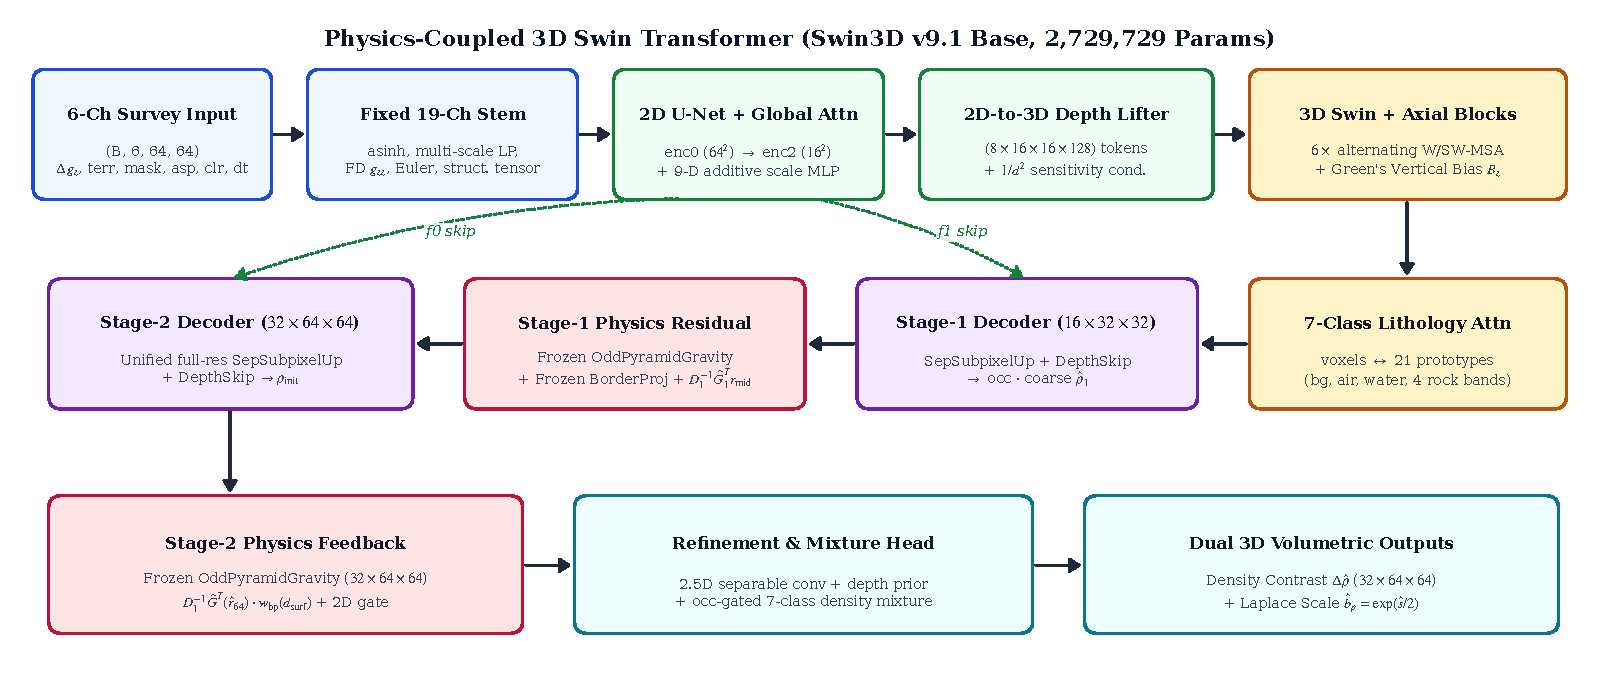
\includegraphics[width=\textwidth]{figures/fig1_architecture.pdf}
  \caption{End-to-end schematic of \texttt{Swin3D v9.1} Base (\valVNineOneParamsExact{} parameters). Physical structure enters at four points: the fixed 19-channel analytical derivative stem, $1/d^2$ depth-conditioned 2D-to-3D lifting, learnable vertical Green's attention bias $B_z$, and two frozen coarse-to-fine spatial-pyramid forward/adjoint residual stages (\texttt{OddPyramidGravity}).}
  \label{fig:arch}
\end{figure*}

Figure~\ref{fig:arch} depicts the \texttt{Swin3D v9.1} (\texttt{PotentialFieldTransformer3DV9}) forward pass; complete channel dimensions and hyperparameters are tabulated in Appendix~\ref{app:specs}.

\paragraph{Multi-Channel Survey Conditioning and Fixed Physics Stem.}
The network accepts a 6-channel $(B, 6, 64, 64)$ surface tensor encoding: (1) observed or border-detrended $\Delta g_z$ $[\text{mGal}]$, (2) normalized terrain depth $z_{\mathrm{terr}} / Z_{\max} \in [0, 0.25]$, (3) valid observation station mask $\mathbf{v}_{\mathrm{mask}} \in [0,1]$, (4) log cell aspect ratio $\ln(\Delta z / \Delta x)$, (5) normalized sensor clearance $\tilde{h} = h / 50\;\text{m}$, and (6) detrending indicator flag ($\text{dt} \in [0,1]$). Normalizing $\Delta g_z$ by its peak magnitude $s = \max|\Delta g_z|$, a \emph{fixed analytical} 19-channel stem (zero learnable parameters; Table~\ref{tab:app_stem}) transforms the normalized anomaly into $\operatorname{asinh}$ compression, four multi-scale box-filter regional/residual bands, two $3\times 3$ finite-difference Laplacian vertical-derivative proxies $g_{zz} = -(g_{xx} + g_{yy})$, horizontal gradient magnitude, tilt-angle and Euler structural-depth proxies, structure-tensor coherence and strike orientation, terrain slope/curvature, station mask, and detrend flag. Concurrently, a 9-dimensional continuous metadata vector---encoding log and bounded peak gravity amplitude relative to a reference Bouguer slab, normalized $\max$ and $\min$ gravity polarity ratios, mean and standard deviation of terrain relief, mean log-aspect, $\ln(1 + \bar{h}/50\,\text{m})$, and mean detrend flag---feeds a 2-layer conditioning MLP (\texttt{scale\_mlp}) whose \emph{additive} embeddings modulate the 2D bottleneck, 3D token volume, lithology prototypes, and full-resolution decoder.

\paragraph{2D Encoder, $1/d^2$ Depth Lifter, and 3D Swin + Axial Backbone.}
A 2D convolutional encoder compresses features from $64 \times 64$ (\texttt{enc0}, 32 channels) through $32\times 32$ (\texttt{enc1}, 64 channels) to $16 \times 16$ (\texttt{enc2}, 128 channels) followed by a global 2D self-attention block, retaining skip maps $(\mathbf{f}_0, \mathbf{f}_1)$. A linear Depth Lifter expands \texttt{enc2} across $D_p = 8$ coarse depth slabs into an $(8 \times 16 \times 16 \times 128)$ volumetric token grid, additively conditioned on normalized depth below terrain $d_{\mathrm{surf}}$, absolute depth, analytical sensitivity proxy $0.04 / (d_{\mathrm{surf}} + 0.08\,\tilde{h} + 0.12)^2$, clearance, and log-aspect. Six alternating 3D Swin Transformer blocks (\texttt{W-MSA} and shifted \texttt{SW-MSA} with $4\times 4$ lateral windows across full depth; \citealp{liu2021swin}) interleaved with separable axial global attention layers exchange information across both local 3D contacts and full domain apertures. Every vertical self-attention logit in head $h$ receives a learnable additive vertical Green's bias (\texttt{GreensVerticalBias}):
\begin{equation}
  B_{z,h}(z_i, z_j) = \left(g_h + a_h \frac{z_j - z_i}{D_p}\right) \frac{1}{1 + \operatorname{softplus}(\gamma_h)\,(z_i - z_j)^2},
  \label{eq:gvb}
\end{equation}
parameterized purely by vertical slab index offsets $(z_i, z_j)$ with learnable per-head gain $g_h$, asymmetry $a_h$, and decay rate $\gamma_h$ initialized to mirror $1/(1 + 0.1\,(z_i - z_j)^2)$ vertical coupling.

\paragraph{7-Class Lithology Prototype Cross-Attention.}
Volumetric tokens interact via bidirectional cross-attention with $21$ learnable lithology prototypes partitioned evenly ($3$ sub-prototypes each) across 7 canonical density regimes: host background ($\Delta\rho = 0$), air cavity ($-2.67\;\text{g/cm}^3$), water-filled void ($-1.67$), light/coal/\allowbreak evaporite ($[-1.60, -0.80]$), sediment/\allowbreak waste ($[-0.85, -0.03]$), mafic/\allowbreak intermediate ($[+0.03, +0.80]$), and dense ore/\allowbreak ultramafic ($[+0.75, +1.95]\;\text{g/cm}^3$).

\paragraph{Two-Stage Coarse-to-Fine Physics Residual Refinement.}
Decoupling coarse volumetric reasoning from unified full-resolution decoding with closed-loop frozen physics feedback proceeds in two stages:
\begin{enumerate}[leftmargin=1.4em,itemsep=0.25em]
  \item \emph{Stage-1 Residual ($16\times 32\times 32$):} A separable subpixel decoder conditioned on $\mathbf{f}_1$ predicts coarse occupancy and preliminary density $\Delta\hat{\rho}_1$. A frozen half-resolution \texttt{OddPyramidGravity} operator $\tilde{\mathbf{G}}_1$ and frozen 1-cell border-ring plane projector \texttt{BorderProjectorConv} compute the peak-normalized masked residual $\hat{\mathbf{r}}_{\mathrm{mid}} = \mathbf{v}_{\mathrm{mask}}\odot\bigl(\hat{\mathbf{d}}_{\mathrm{obs}} - \mathcal{P}_{\mathrm{det}}^{\mathrm{dt}}(\tilde{\mathbf{G}}_1\Delta\hat{\rho}_1 / s)\bigr)$ (with $\hat{\mathbf{d}}_{\mathrm{obs}} = \mathbf{d}_{\mathrm{obs}}/s$ and $\mathcal{P}_{\mathrm{det}}^{\mathrm{dt}}$ applying border detrending when $\text{dt}=1$), feeding back the sensitivity-normalized adjoint back-projection $D_{1,\mathrm{mid}}^{-1}\tilde{\mathbf{G}}_1^T \hat{\mathbf{r}}_{\mathrm{mid}}$ alongside 2D residual features gated by depth.
  \item \emph{Stage-2 Unified Decoding \& Physics Back-Projection ($32\times 64\times 64$):} Rather than splitting depth bands into disjoint decoders (\texttt{v7}/\texttt{v8}), \texttt{v9.1} decodes in a single unified $(32\times 64\times 64)$ grid using $\mathbf{f}_0$ skips to produce $\Delta\rho_{\mathrm{init}}$, evaluates the full-resolution normalized masked residual $\hat{\mathbf{r}}_{64}$, and injects sensitivity-normalized, depth-amplified adjoint gradients:
  \begin{equation}
  \begin{aligned}
    \Delta_{\mathrm{phys}}(x,y,z) &= D_1^{-1}\tilde{\mathbf{G}}^T(\hat{\mathbf{r}}_{64}) \cdot w_{\mathrm{bp}}\bigl(d_{\mathrm{surf}}(x,y,z)\bigr), \\
    w_{\mathrm{bp}}(d_{\mathrm{surf}}) &= 1 + \operatorname{softplus}(\beta_{\mathrm{bp}})\,d_{\mathrm{surf}}\bigl(1 + 2\,d_{\mathrm{surf}}\bigr),
  \end{aligned}
    \label{eq:bp_weight}
  \end{equation}
  where $d_{\mathrm{surf}}(x,y,z) = \max\bigl(0,\, z/Z_{\max} - z_{\mathrm{terr}}(x,y)/Z_{\max}\bigr) \in [0,1]$ is dimensionless normalized depth below terrain, $D_1 = \operatorname{diag}\!\bigl(\max(0.15,\, \tilde{\mathbf{G}}^T\mathbf{v}_{\mathrm{mask}})\bigr)$ is clamped diagonal column-sensitivity normalization, and $\beta_{\mathrm{bp}}$ is learned. Final 2.5D separable convolution refinement outputs both the predicted density contrast $\Delta\hat{\rho}$ (occupancy-gated mixture across the 7 lithology bands plus a $\pm 0.10\;\text{g/cm}^3$ residual head) and an 8-cue heteroscedastic log-scale head predicting the Laplace scale parameter $\hat{b}_\rho = \exp(\hat{s}/2)$ with $\hat{s} \in [-8, 4]$.
\end{enumerate}

The base configuration evaluated throughout this paper contains \valVNineOneParamsExact{} (\valVNineOneParams{}) trainable parameters; modular presets also define \texttt{slim} (\valVNineOneSlimParams{}) and \texttt{heavy} (\valVNineOneHeavyParams{}) capacities.

\subsection{Compound Physics-Informed Objective and Laplace $\beta$-NLL}

Training a 3D gravity inverter solely with voxel-wise MSE collapses predictions toward smooth low-amplitude blobs. We minimize a weighted deep-supervision objective combining structural geometry, lithology semantics, interior distance regularization, intermediate coarse/initial supervision, forward gravity consistency, and calibrated Laplace uncertainty:
\begin{equation}
\begin{aligned}
  \mathcal{L}_{\mathrm{total}} &= \mathcal{L}_{\mathrm{struct}}(\Delta\hat{\rho}, \Delta\rho)
  + \lambda_{\mathrm{cls}}\,\mathcal{L}_{\mathrm{cls}}(\hat{\mathbf{p}}_{\mathrm{cls}}, \mathbf{c})
  + \lambda_{\mathrm{coh}}\,\mathcal{L}_{\mathrm{coh}}(\hat{\mathbf{p}}_{\mathrm{cls}}, \Delta\hat{\rho}, \Delta\rho) \\
  &\quad + \mathcal{L}_{\mathrm{edt}}(\hat{\mathbf{e}}_{\mathrm{edt}}, \mathbf{e}_{\mathrm{edt}})
  + \lambda_{\mathrm{coarse}}\,\mathcal{L}_{\mathrm{coarse}}(\Delta\hat{\rho}_1, \Delta\rho)
  + \lambda_{\mathrm{init}}\,\mathcal{L}_{\mathrm{init}}(\Delta\rho_{\mathrm{init}}, \Delta\rho) \\
  &\quad + \lambda_{\mathrm{data}}\,\mathcal{L}_{\mathrm{data}}(\mathbf{G}\Delta\hat{\rho}, \mathbf{d}_{\mathrm{clean}})
  + \lambda_{\mathrm{nll}}\,\mathcal{L}_{\beta\text{-NLL}}(\Delta\hat{\rho}, \hat{s}, \Delta\rho),
\end{aligned}
  \label{eq:loss_total}
\end{equation}
with fixed weights $\lambda_{\mathrm{cls}}=0.25$, $\lambda_{\mathrm{coh}}=0.12$, $\lambda_{\mathrm{coarse}}=0.20$, $\lambda_{\mathrm{init}}=0.10$, $\lambda_{\mathrm{data}}=0.50$, and $\lambda_{\mathrm{nll}}=0.06$. Here $\hat{\mathbf{p}}_{\mathrm{cls}} \in [0,1]^{7\times N_m}$ are predicted 7-class voxel probabilities, $\mathbf{c} \in \{0,\dots,6\}^{N_m}$ are ground-truth lithology indices, and $\hat{\mathbf{e}}_{\mathrm{edt}}$ predicts a 4-step morphological interior distance proxy $\mathbf{e}_{\mathrm{edt}}$ to prevent hollow centers inside thick bodies. Full sub-term formulas for $\mathcal{L}_{\mathrm{struct}}$ (depth-weighted foreground $L_1$/$L_2$, distance-weighted relative $L_1$, opposite-sign halo suppression, Tanimoto + per-unit Smooth 3D IoU, 3D face-gradient sharpness, multi-band mass conservation, amplitude consistency, and Zhdanov MGS matching), $\mathcal{L}_{\mathrm{cls}}$, $\mathcal{L}_{\mathrm{coh}}$, and $\mathcal{L}_{\mathrm{data}}$ (Charbonnier relative amplitude and horizontal gradient misfit under the exact operator $\mathbf{G}$) are given in Appendix~\ref{app:specs}.

For aleatoric uncertainty estimation, \texttt{Swin3D v9.1} minimizes a \emph{zone-stratified Laplace $\beta$-NLL} objective adapting \citet{seitzer2022betanll} and \citet{kendall2017} to $L_1$ residuals, preventing background sparsity from overwhelming foreground calibration:
\begin{equation}
  \mathcal{L}_{\beta\text{-NLL}} = \sum_{r \in \{\mathrm{fg},\,\mathrm{bd},\,\mathrm{far}\}} \omega_r \left[
    \frac{1}{|\Omega_r|} \sum_{j \in \Omega_r} \operatorname{sg}\!\left(\hat{b}_{\rho,j}^{\beta_{\mathrm{NLL}}}\right)
    \left( \frac{|\Delta\hat{\rho}_j - \Delta\rho_j|}{\hat{b}_{\rho,j}} + \ln\hat{b}_{\rho,j} + 4 \right)
  \right], \qquad \beta_{\mathrm{NLL}} = 0.5,
  \label{eq:betanll}
\end{equation}
where $\hat{b}_{\rho,j} = \exp(\hat{s}_j/2)$, $\operatorname{sg}(\cdot)$ stops gradients through the weighting factor, and $\Omega_{\mathrm{sub}}$ is partitioned into ground-truth foreground $\Omega_{\mathrm{fg}}$ ($\omega_{\mathrm{fg}} = 0.50$), the 3-voxel dilated boundary shell $\Omega_{\mathrm{bd}}$ ($\omega_{\mathrm{bd}} = 0.35$), and far host rock $\Omega_{\mathrm{far}}$ ($\omega_{\mathrm{far}} = 0.15$). Under a well-calibrated Laplace predictive distribution $p(e) = (2\hat{b}_\rho)^{-1}\exp(-|e|/\hat{b}_\rho)$, the theoretical expected MAE equals $\hat{b}_\rho$, RMSE equals $\sqrt{2}\,\hat{b}_\rho$, and $1$-scale coverage $P(|e| \le \hat{b}_\rho)$ equals $1 - e^{-1} \approx 63.2\%$. Figure~\ref{fig:train_abl}(b) displays the empirical weighted share of each component in~\eqref{eq:loss_total} at best epoch~\valVNineOneEp{}.

\subsection{Procedural Data Generation, Training Protocol, and Classical Solvers}
\label{sec:classical}

An on-the-fly procedural generator synthesizes 3D lithology and density volumes inside active terrain subvolumes ($\le 25\%$ relief fraction) drawing 1--4 interacting archetypes from compact blocks, elliptical lenses, dipping mafic dykes, subvertical stocks, buried basins, cavities, folded undulating strata, and nested core--halo complexes across the 7 lithology ranges. Training surveys span ground clearance ($h \in [0.30, 2.0]$\,m, 67\% probability), airborne relief drapes ($h \in [2.0, 160.0]$\,m, 33\%), missing-station masks with harmonic infill, anisotropic cell aspect ratios $\Delta z/\Delta x \in \{0.55, 0.75, 1.0, 1.20, 1.40\}$, 3D petrophysical voxel clutter ($8\%$ internal heterogeneity), $0.5\text{--}4\%$ station noise, and raw vs.\ border-detrended regional modes, augmented by exact dihedral $D_4$ horizontal symmetries \citep{cerovsky_mod3d}. Training runs in FP32 PyTorch MPS on a single consumer MacBook Air (Apple~M4, 10-core CPU, 32\,GB unified memory) with batch size~8, 200 optimizer steps per epoch, AdamW ($\text{lr}=5\times 10^{-4}$; \citealp{loshchilov2019adamw}), cosine learning-rate annealing, a 25-epoch difficulty curriculum, and exponential moving average (EMA) weight averaging. Validation and best-checkpoint selection during training used fixed seed~\valTrainValSeed{}; the flagship checkpoint archived in \texttt{.inv/paper/models/v9.1\_hard\_best.pt} corresponds to best epoch~\valVNineOneEp{}. All headline test benchmarks in Section~\ref{sec:experiments} use a strictly disjoint held-out test seed (\valTestSeed{}).

For head-to-head comparison on identical $64\times 64\times 32$ topographic forward operators, we run a pure Python/\allowbreak PyTorch FFT implementation (\texttt{scripts/\allowbreak classical\_baselines.py}) of regularized Zhdanov inversion \citep{tikhonov1977,last1983,li1998,portniaguine1999,zhdanov2002}. At outer IRLS iteration $k$, the solver minimizes the sensitivity-weighted quadratic majorizer:
\begin{equation}
\begin{aligned}
  \Phi^{(k)}(\mathbf{m}) &= \left\|\mathbf{W}_d \bigl(\mathbf{G}\mathbf{m} + \mathbf{b}^{(k)} - \mathbf{d}_{\mathrm{obs}}\bigr)\right\|_2^2 \\
  &\quad + \alpha^{(k)} \left(
    \mu_{\mathrm{MS}} \sum_{j \in \Omega_{\mathrm{sub}}} w_j^2 W_{e,j}^{(k)2} m_j^2
    + \mu_{\mathrm{MGS}} \sum_{(a,b) \in \mathcal{E}_{\mathrm{sub}}} A_{ab}\, w_{ab}^2 W_{f,ab}^{(k)2} (m_b - m_a)^2
  \right),
\end{aligned}
  \label{eq:focusing_obj}
\end{equation}
where $\mathbf{W}_d = \sigma_d^{-1}\operatorname{diag}(\mathbf{v}_{\mathrm{mask}})$, $\mathbf{b}^{(k)}$ is the perimeter-fitted \texttt{BackgroundBasis} trend when detrending is enabled, $w_j^2 = (S_j^2 / S_{\max}^2)^\gamma$ is normalized integrated column sensitivity ($S_j^2 = \sum_i G_{ij}^2$), $\mathcal{E}_{\mathrm{sub}}$ denotes adjacent active interior voxel faces with normalized face area $A_{ab}$ and face-averaged sensitivity $w_{ab}^2 = \frac{1}{2}(w_a^2 + w_b^2)$, and box bounds $\Delta\rho \in [-2.67, +1.95]\;\text{g/cm}^3$ are projected after each Jacobi-preconditioned conjugate-gradient solve.
\begin{itemize}[leftmargin=1.4em,itemsep=0.2em]
  \item \textbf{Depth-Weighted Tikhonov $L_2$ ($\gamma = 0.50$):} Sets uniform quadratic weights $W_{e,j}^{(k)} = W_{f,ab}^{(k)} = s_{\mathrm{ref}}^{-1}$ (reference density scale $s_{\mathrm{ref}} = 0.25\;\text{g/cm}^3$) with standard Zhdanov sensitivity exponent $\gamma = 0.50$ ($w_j \propto S_j^{1/2}$), mild smoothness weight ($\mu_{\mathrm{MS}}=1.0$, $\mu_{\mathrm{MGS}}=0.25$), and up to 10 Morozov discrepancy cooling iterations targeting $\chi_{\mathrm{rms}} = \sqrt{\chi^2_{\mathrm{red}}} \in [0.95, 1.05]$.
  \item \textbf{Portniaguine--Zhdanov Focusing IRLS ($\gamma = 0.75$):} Uses reweighted minimum-support and minimum-gradient-support weights $W_{e,j}^{(k)} = (w_j^2 m_j^{(k-1)2} + e_k^2)^{-1/2}$ and $W_{f,ab}^{(k)} = (w_{ab}^2 (m_b^{(k-1)} - m_a^{(k-1)})^2 + e_k^2)^{-1/2}$ ($\mu_{\mathrm{MS}}=\mu_{\mathrm{MGS}}=1.0$, $\gamma = 0.75$), cooling $e_k$ from $1.0$ to $0.01$ relative amplitude over 12 iterations targeting $\chi_{\mathrm{rms}} \in [0.94, 1.06]$.
\end{itemize}

%======================================================================
\section{Synthetic Experiments}
\label{sec:experiments}
%======================================================================

\subsection{Evaluation Protocol and Exact Metric Definitions}

All quantitative evaluations run deterministically on CPU (\valCpuThreads{} threads) from archived checkpoints in \texttt{.inv/paper/models/} on held-out seeds disjoint from training validation seed~\valTrainValSeed{}. Every metric matches the exact code definitions in \texttt{evaluate.py} and \texttt{eval\_paper\_v9\_1.py}:
\begin{itemize}[leftmargin=1.4em,itemsep=0.25em]
  \item \textbf{Smooth 3D IoU} ($\uparrow$): Sign-consistent soft Jaccard index comparing the binary ground-truth support against a smooth $[0,1]$ support ramp of $|\Delta\hat{\rho}|$ normalized per geological unit at $50\%$ of local target amplitude.
  \item \textbf{Global RMSE \& FG-RMSE} ($\downarrow$, $[\text{g/cm}^3]$): Root-mean-square density error over all active subsurface voxels $\Omega_{\mathrm{sub}}$ (RMSE) and restricted strictly to ground-truth anomalous target voxels $\Omega_{\mathrm{fg}}$ (FG-RMSE).
  \item \textbf{3D SSIM \& $\text{SSIM}_{d_3}$} ($\uparrow$): Gaussian-windowed 3D structural similarity \citep{wang2004ssim} averaged over $\Omega_{\mathrm{sub}}$ ($\text{SSIM}_{\mathrm{3D}}$) and restricted to the \emph{3-voxel morphologically dilated foreground shell} ($\text{SSIM}_{d_3}$), eliminating background inflation.
  \item \textbf{Vertical Centroid Error $|\Delta z|$} ($\downarrow$, $[\text{m}]$): Mass-weighted average over per-component 3D Voronoi partitions (within a $7\times 7$ laterally dilated same-sign column thresholded at $20\%$ peak amplitude) of $|z_{\mathrm{pred}} - z_{\mathrm{true}}|$. For scatter diagnostics (Figure~\ref{fig:calib}(c)), we also report scene-level global centroid depth $z_{\mathrm{pred}}$ vs.\ $z_{\mathrm{true}}$ and mean signed depth bias $\overline{z_{\mathrm{pred}} - z_{\mathrm{true}}}$.
  \item \textbf{Foreground Mass Recovery Ratio (Amp.)} ($\to 1$): Sign-consistent mass recovery inside the ground-truth body support, $\sum_{j \in \Omega_{\mathrm{fg}}} \Delta\hat{\rho}_j \operatorname{sgn}(\Delta\rho_j) / \sum_{j \in \Omega_{\mathrm{fg}}} |\Delta\rho_j|$, diagnosing amplitude underestimation.
  \item \textbf{Relative Gravity Misfit \& $\chi^2_{\mathrm{red}}$}: Relative surface $L_2$ misfit $\|\mathbf{r}\|_2 / \|\mathbf{d}_{\mathrm{eff}}\|_2$ [\%] evaluated under the exact forward and detrending operator, plus reduced chi-squared $\chi^2_{\mathrm{red}} = \frac{1}{N_{\mathrm{valid}}}\|\mathbf{v}_{\mathrm{mask}}\odot\mathbf{r}/\sigma_d\|_2^2$ ($N_{\mathrm{valid}}=\sum_i v_{\mathrm{mask},i}$) when noise $\sigma_d > 0$ is known.
  \item \textbf{Laplace Calibration Metrics}: Pooled Area Under the Risk--Coverage Curve ($\mathrm{AURC}\downarrow$, cumulative mean $|\Delta\hat{\rho}-\Delta\rho|$ ordered by $\hat{b}_\rho$), Spearman rank correlation on foreground voxels ($\rho_{\mathrm{fg}}$) and all subsurface voxels ($\rho_{\mathrm{all}}$), foreground $1$-$b$ coverage $P(|\Delta\hat{\rho}-\Delta\rho| \le \hat{b}_\rho)$ (ideal Laplace $63.2\%$), and 1-cell boundary calibration ratio $\overline{\hat{b}_\rho}_{\partial\mathcal{B}} / \overline{|\Delta\hat{\rho}-\Delta\rho|}_{\partial\mathcal{B}}$ (ideal Laplace $1.00$).
\end{itemize}

\subsection{Held-Out Multi-Regime Test and Chronological Progression}

\begin{table}[t]
\centering
\caption{Held-out multi-regime test performance of \texttt{Swin3D v9.1} (\valVNineOneParams{} parameters, epoch~\valVNineOneEp{}) across four stratified survey regimes ($N=\valNBucketTotal{}$ scenes, disjoint test seed~\valTestSeed{}). Columns report regime weight (Wt.), Smooth 3D IoU (mean\,$\pm$\,std), subsurface RMSE and foreground target RMSE (FG-RMSE), 3-voxel dilated foreground SSIM ($\text{SSIM}_{d_3}$), vertical centroid error $|\Delta z|$ (mean\,$\pm$\,std), foreground mass recovery ratio (Amp.), effective gravity misfit, and Laplace $1$-$b$ coverage (ideal $63.2\%$).}
\label{tab:v91_buckets}
\small
\setlength{\tabcolsep}{4pt}
\resizebox{\textwidth}{!}{%
\begin{tabular}{lccccccccc}
\toprule
Regime Bucket & Wt. & IoU $\uparrow$ & RMSE $\downarrow$ & FG-RMSE $\downarrow$ & $\text{SSIM}_{d_3}$ $\uparrow$ & $|\Delta z|$ [m] $\downarrow$ & Amp. $\to 1$ & Misfit [\%] $\downarrow$ & $1$-$b$ Cov. \\
\midrule
Ground Clean & 0.35 & 0.531\,$\pm$\,0.109 & 0.043 & 0.360 & 0.591 & 29.3\,$\pm$\,24.1 & 0.653 & 3.98 & 63.0\% \\
Hard-Large Detrended & 0.35 & 0.658\,$\pm$\,0.176 & 0.091 & 0.283 & 0.569 & 46.4\,$\pm$\,40.5 & 0.755 & 6.83 & 63.0\% \\
Airborne Relief Drape & 0.15 & 0.633\,$\pm$\,0.164 & 0.067 & 0.308 & 0.593 & 36.7\,$\pm$\,23.2 & 0.734 & 5.97 & 73.7\% \\
Multi-Aspect ($\Delta z/\Delta x$) & 0.15 & 0.702\,$\pm$\,0.169 & 0.072 & 0.257 & 0.608 & 39.2\,$\pm$\,53.4 & 0.807 & 4.86 & 65.1\% \\
\midrule
\textbf{Weighted Composite} & 1.00 & \textbf{0.617\,$\pm$\,0.164} & \textbf{0.067} & \textbf{0.310} & \textbf{0.586} & \textbf{37.9\,$\pm$\,36.0} & \textbf{0.724} & \textbf{5.41} & \textbf{64.9\%} \\
\bottomrule
\end{tabular}%
}
\end{table}


Table~\ref{tab:v91_buckets} reports \texttt{Swin3D v9.1} (epoch~\valVNineOneEp{}) performance across four stratified regimes totaling $N=\valNBucketTotal{}$ held-out scenes (disjoint test seed~\valTestSeed{}). The model achieves a weighted composite Smooth 3D IoU of $\valCompIoU{} \pm \valCompIoUStd{}$, $|\Delta z|$ of $\valCompDz{} \pm \valCompDzStd{}$\,m (sub-voxel relative to the $50$\,m grid spacing), $\text{SSIM}_{\mathrm{3D}} = \valCompSSIM{}$ ($\text{SSIM}_{d_3} = \valCompSSIMd{}$), mass recovery of \valCompAmp{}, FG-RMSE of \valCompFGRMSE{}\,g/cm$^3$, global RMSE of \valCompRMSE{}\,g/cm$^3$, opposite-sign halo energy of $\valCompHalo{}\times 10^{-4}$, and \valCompMisfit{}\% gravity misfit. Performance holds robustly across \emph{Hard-Large Detrended} (IoU \valHLIoU{}, $|\Delta z| = \valHLDz{}$\,m), \emph{Airborne Relief Drape} ($h \in [2, 160]$\,m over up to 25\% topography; IoU \valAirIoU{}, $|\Delta z| = \valAirDz{}$\,m), and \emph{Multi-Aspect} anisotropy (IoU \valMAIoU{}, $|\Delta z| = \valMADz{}$\,m).

\begin{figure*}[t]
  \centering
  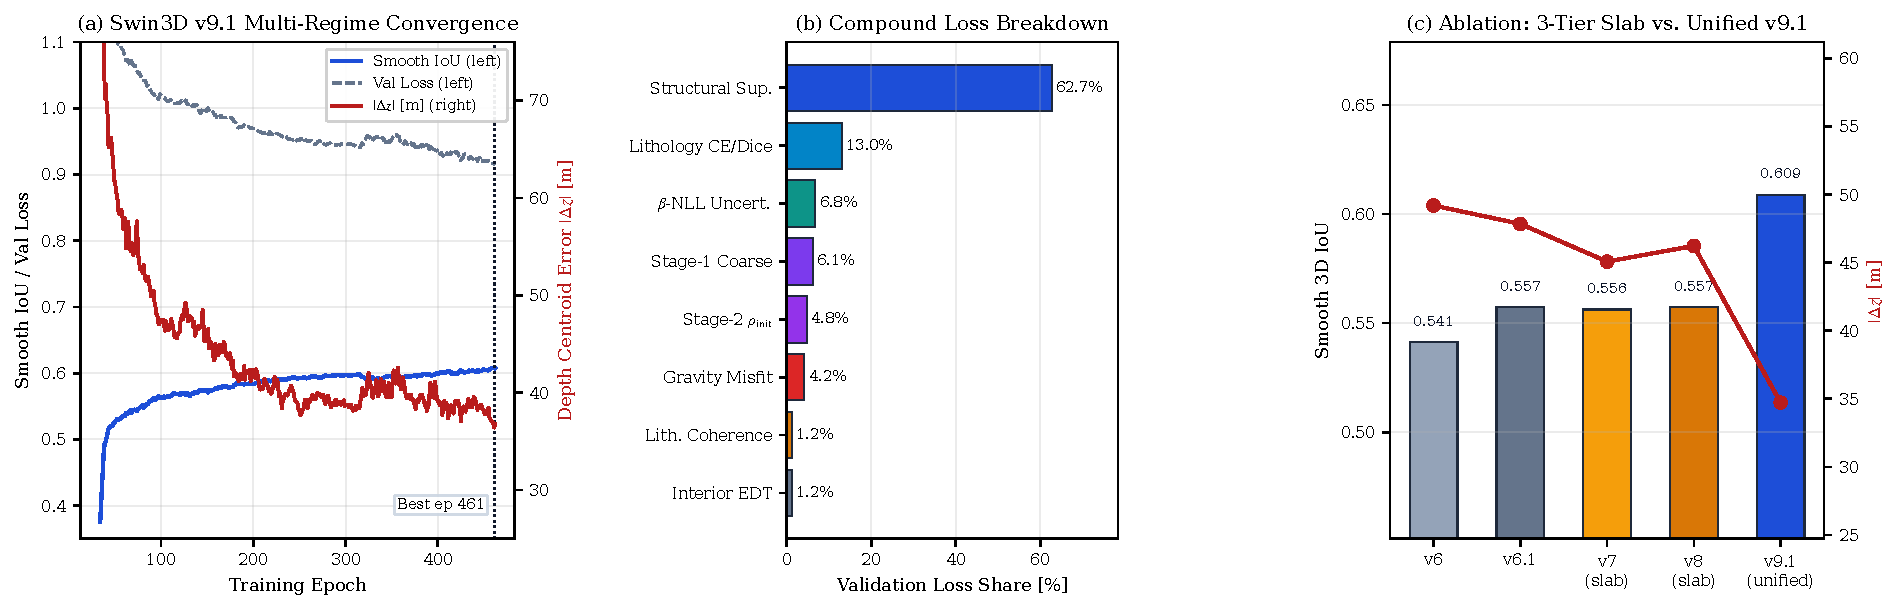
\includegraphics[width=\textwidth]{figures/fig2_training_ablation.pdf}
  \caption{Training dynamics and chronological architecture progression. (a) Validation Smooth 3D IoU, total loss, and vertical centroid error $|\Delta z|$ of \texttt{Swin3D v9.1} across logged epochs~34--514 (best checkpoint at epoch~\valVNineOneEp{}). (b) Relative weighted shares of the compound validation loss components at epoch~\valVNineOneEp{}. (c) Held-out multi-regime evaluation ($N=\valNAblBucket{}$, seed~\valTestSeed{}) across historical model generations \texttt{v6}--\texttt{v9.1} with checkpoint epochs labeled and a dotted line marking \texttt{v9.1} validation IoU at matched epoch~\valMatchedEp{} (\valMatchedIoU{}).}
  \label{fig:train_abl}
\end{figure*}

\begin{table}[t]
\centering
\caption{Controlled architectural ablation across identical seeded validation sets. Panel~A evaluates the 4-bucket realistic survey suite ($N=\valNAblBucket{}$); Panel~B evaluates the clean ground benchmark ($N=\valNCleanStd{}$ standard + $\valNCleanHard{}$ hard scenes). Bold marks best per panel.}
\label{tab:ablation}
\small
\setlength{\tabcolsep}{4pt}
\resizebox{\textwidth}{!}{%
\begin{tabular}{lcllcccccc}
\toprule
Model & Params & Ch. & Key Configuration & IoU $\uparrow$ & $|\Delta z|$ [m] $\downarrow$ & Amp. $\to 1$ & Misfit [\%] $\downarrow$ & RMSE $\downarrow$ & $\text{SSIM}_{d_3}$ $\uparrow$ \\
\midrule
\multicolumn{10}{l}{\textit{Panel A: Multi-Regime Realistic Survey Suite (ground, hard-detrended, airborne drape, multi-aspect)}} \\
\texttt{v6} & 2.73M & 5 & 5-ch + 2-Stage Unified & 0.541 & 49.2 & 0.648 & 11.85 & 0.074 & 0.499 \\
\texttt{v6.1} & 2.73M & 5 & 5-ch + GVB + Smooth IoU & 0.557 & 47.8 & 0.684 & 9.92 & 0.073 & 0.520 \\
\texttt{v7} & 2.86M & 6 & 6-ch + 3-Tier Slab & 0.556 & 45.1 & 0.682 & 9.36 & 0.072 & 0.524 \\
\texttt{v8} & 2.86M & 6 & 6-ch + 3-Tier Unrolled & 0.557 & 46.2 & 0.675 & 7.75 & 0.071 & 0.527 \\
\textbf{\texttt{v9.1}} (ours) & 2.73M & 6 & 6-ch + Unified + Coh. & \textbf{0.609} & \textbf{34.7} & \textbf{0.721} & \textbf{5.37} & \textbf{0.067} & \textbf{0.563} \\
\midrule
\multicolumn{10}{l}{\textit{Panel B: Clean Ground Survey Benchmark (standard + hard composite targets)}} \\
\texttt{v3} & 2.70M & 2 & 2-ch + Prototypes & 0.566 & 22.4 & 0.738 & 7.28 & 0.048 & 0.661 \\
\texttt{v5.2} & 2.73M & 5 & 5-ch + GVB + NLL & 0.575 & 22.2 & \textbf{0.751} & 6.56 & 0.048 & 0.669 \\
\texttt{v8} (clean) & 2.86M & 6 & 6-ch + 3-Tier Unrolled & 0.369 & 58.9 & 0.485 & 9.94 & 0.060 & 0.504 \\
\texttt{v9} (clean) & 2.73M & 6 & 6-ch + Unified Decoder & 0.567 & 23.0 & 0.733 & 4.38 & 0.048 & 0.664 \\
\textbf{\texttt{v9.1}} (clean) & 2.73M & 6 & 6-ch + Unified + Coh. & \textbf{0.576} & \textbf{21.5} & 0.742 & \textbf{4.09} & \textbf{0.047} & \textbf{0.673} \\
\texttt{v9.1} (zero-shot xfer) & 2.73M & 6 & 6-ch Hard Zero-Shot & 0.541 & 23.2 & 0.677 & 4.30 & 0.048 & 0.646 \\
\bottomrule
\end{tabular}%
}
\end{table}


Table~\ref{tab:ablation} and Figure~\ref{fig:train_abl}(c) trace chronological model iterations across identical held-out test seeds without post-hoc tuning. Because historical runs terminated at different training budgets (explicitly listed in the Ep.\ column), we carefully separate architectural effects from training duration:
\begin{itemize}[leftmargin=1.4em,itemsep=0.25em]
  \item On the realistic 4-regime suite (Panel~A, $N=\valNAblBucket{}$), adding \texttt{GreensVerticalBias} and Smooth 3D IoU (\texttt{v6} $\to$ \texttt{v6.1}, warm-started from \texttt{v6}) raises IoU from \valAblVSixIoU{} to \valAblVSixOneIoU{} and reduces misfit from \valAblVSixMisfit{}\% to \valAblVSixOneMisfit{}\%. Adding 6-channel survey conditioning with 3-tier slab-split decoders (\texttt{v7}, ep~99; \texttt{v8}, ep~97) lowers misfit further to \valAblVEightMisfit{}\% and reaches \valAblVSevenIoU{}--\valAblVEightIoU{} IoU ($|\Delta z| = \valAblVEightDz{}$--\valAblVSevenDz{}\,m). At epoch~\valVNineOneEp{}, unified \texttt{v9.1} attains \valAblVNineOneIoU{} IoU, $|\Delta z| = \valAblVNineOneDz{}$\,m, $\text{SSIM}_{d_3} = \valAblVNineOneSSIMd{}$, and \valAblVNineOneMisfit{}\% misfit. Crucially, examining \texttt{v9.1}'s logged trajectory at \emph{matched epoch~\valMatchedEp{}} yields validation IoU \valMatchedIoU{} and $|\Delta z| = \valMatchedDz{}$\,m---comparable to \texttt{v8} at epoch~97---demonstrating that \textbf{extended multi-regime training (\valVNineOneEp{} vs.\ \valMatchedEp{} epochs) accounts for the majority of Panel~A's final IoU gap}, while unified Stage-2 decoding eliminates slab-boundary complexity and stabilizes long-horizon convergence.
  \item On clean ground benchmarks (Panel~B, $N=\valNCleanStd{}$ standard + $\valNCleanHard{}$ hard scenes), unified \texttt{v9} (ep~119, IoU \valCleanVNineIoU{}) and \texttt{v9.1} (ep~\valVNineOneCleanEp{}, IoU \valCleanVNineOneIoU{}, $|\Delta z|=\valCleanVNineOneDz{}$\,m, \valCleanVNineOneMisfit{}\% misfit) clearly outperform both \texttt{v3} (\valCleanVThreeIoU{}) and \texttt{v5.2} (\valCleanVFiveTwoIoU{}) at comparable training budgets (118--153 epochs), while the early-stopped 3-tier \texttt{v8} run (ep~\valCleanVEightEp{}) lagged at \valCleanVEightIoU{} IoU (\valCleanVEightDz{}\,m). Zero-shot transfer of multi-regime \texttt{v9.1} holds \valCleanHardXferIoU{} IoU (\valCleanHardXferDz{}\,m centroid error) without clean-regime fine-tuning.
\end{itemize}

\subsection{Head-to-Head Comparison Against Classical Solvers}

\begin{figure*}[t]
  \centering
  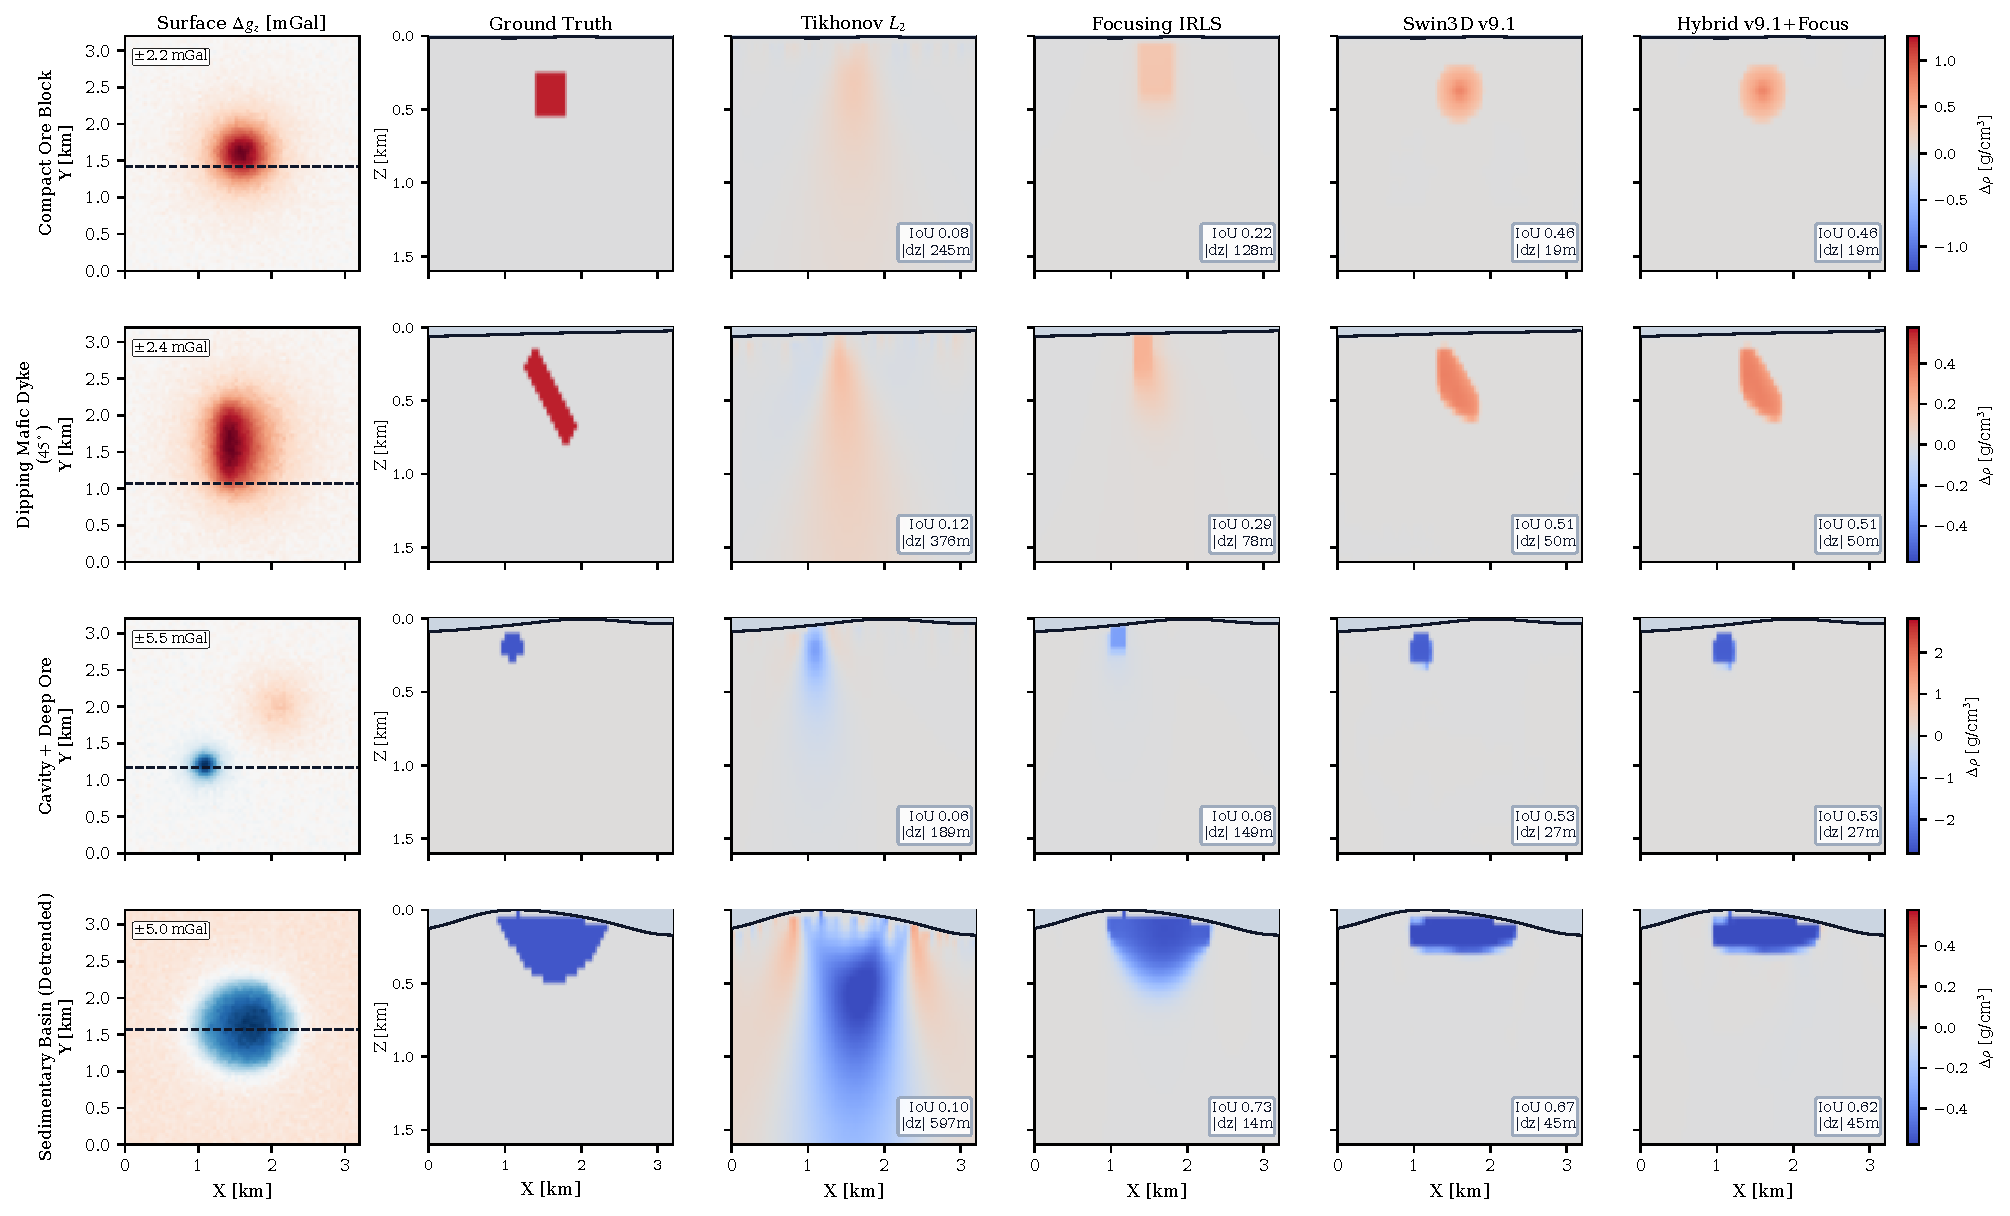
\includegraphics[width=\textwidth]{figures/fig3_canonical_comparison.pdf}
  \caption{Cross-section comparison on four canonical 3D benchmarks (2\% white Gaussian noise). Column~1 shows surface $\Delta g_z$ with color scale and profile trace (dashed line, $Y=1.6$\,km). Columns~2--5 display vertical $X$--$Z$ density cross-sections ($Z=0\text{--}1.6$\,km; grey shading marks air above topography) for ground truth, depth-weighted Tikhonov $L_2$ ($\gamma=0.50$), Focusing IRLS ($\gamma=0.75$), and standalone \texttt{Swin3D v9.1}.}
  \label{fig:canonical}
\end{figure*}

\begin{table}[t]
\centering
\caption{Head-to-head comparison against depth-weighted Tikhonov $L_2$ ($\gamma=0.50$, up to 10 cooling iterations) and Portniaguine--Zhdanov Focusing IRLS ($\gamma=0.75$, 12 iterations) on four canonical 3D benchmarks (single deterministic realizations, 2\% white Gaussian noise, \valCpuThreads{} CPU threads). Bold marks best method per benchmark (ties after rounding both bolded; closest to $1.0$ for Amp.\ and $\chi^2_{\mathrm{red}}$).}
\label{tab:canonical}
\small
\setlength{\tabcolsep}{4pt}
\resizebox{\textwidth}{!}{%
\begin{tabular}{llcccccccc}
\toprule
Benchmark & Method & IoU $\uparrow$ & RMSE $\downarrow$ & $\text{SSIM}_{d_3}$ $\uparrow$ & $|\Delta z|$ [m] $\downarrow$ & Amp. $\to 1$ & Misfit [\%] $\downarrow$ & $\chi^2_{\mathrm{red}}$ $\to 1$ & Time [s] $\downarrow$ \\
\midrule
\multirow{3}{*}{Compact Ore Block} & Tikhonov $L_2$ ($\gamma=0.50$) & 0.091 & 0.060 & 0.124 & 29.5 & 0.154 & 3.60 & 0.76 & 0.76 \\
 & Focusing IRLS ($\gamma=0.75$) & 0.220 & 0.056 & 0.208 & 127.4 & 0.192 & 7.26 & 1.39 & 1.45 \\
 & \texttt{Swin3D v9.1} & \textbf{0.457} & \textbf{0.039} & \textbf{0.528} & \textbf{17.7} & \textbf{0.551} & \textbf{1.00} & \textbf{0.99} & \textbf{0.19} \\
\midrule
\multirow{3}{*}{Dipping Mafic Dyke ($45^\circ$)} & Tikhonov $L_2$ ($\gamma=0.50$) & 0.144 & 0.051 & 0.149 & 165.5 & 0.247 & 3.06 & 0.71 & 2.59 \\
 & Focusing IRLS ($\gamma=0.75$) & 0.290 & 0.047 & 0.199 & 73.3 & 0.292 & 4.25 & 1.23 & 8.38 \\
 & \texttt{Swin3D v9.1} & \textbf{0.520} & \textbf{0.039} & \textbf{0.420} & \textbf{44.4} & \textbf{0.549} & \textbf{3.03} & \textbf{1.12} & \textbf{0.20} \\
\midrule
\multirow{3}{*}{Cavity + Deep Ore} & Tikhonov $L_2$ ($\gamma=0.50$) & 0.064 & 0.080 & 0.302 & \textbf{14.6} & 0.195 & 9.79 & 0.72 & 7.15 \\
 & Focusing IRLS ($\gamma=0.75$) & 0.091 & 0.080 & 0.372 & 93.6 & 0.223 & 15.24 & 1.45 & 11.96 \\
 & \texttt{Swin3D v9.1} & \textbf{0.540} & \textbf{0.062} & \textbf{0.645} & 30.1 & \textbf{0.601} & \textbf{8.53} & \textbf{1.17} & \textbf{0.19} \\
\midrule
\multirow{3}{*}{Sedimentary Basin (Detrended)} & Tikhonov $L_2$ ($\gamma=0.50$) & 0.176 & 0.084 & 0.143 & 449.3 & 0.538 & 3.24 & 0.73 & 4.69 \\
 & Focusing IRLS ($\gamma=0.75$) & \textbf{0.726} & \textbf{0.030} & \textbf{0.618} & \textbf{17.9} & 0.846 & \textbf{2.65} & \textbf{1.06} & 13.85 \\
 & \texttt{Swin3D v9.1} & 0.669 & 0.050 & 0.497 & 44.0 & \textbf{0.874} & 2.94 & 1.10 & \textbf{0.19} \\
\midrule
\multirow{3}{*}{\textbf{Mean (4 Benchmarks)}} & Tikhonov $L_2$ ($\gamma=0.50$) & 0.119 & 0.069 & 0.180 & 164.7 & 0.284 & 4.92 & 0.73 & 3.80 \\
 & Focusing IRLS ($\gamma=0.75$) & 0.332 & 0.053 & 0.349 & 78.0 & 0.388 & 7.35 & 1.28 & 8.91 \\
 & \texttt{Swin3D v9.1} & \textbf{0.547} & \textbf{0.047} & \textbf{0.522} & \textbf{34.0} & \textbf{0.644} & \textbf{3.88} & \textbf{1.10} & \textbf{0.19} \\
\bottomrule
\end{tabular}%
}
\end{table}


Figure~\ref{fig:canonical} and Table~\ref{tab:canonical} compare standalone \texttt{Swin3D v9.1} directly against fair depth-weighted Tikhonov $L_2$ ($\gamma=0.50$) and Portniaguine--Zhdanov Focusing IRLS ($\gamma=0.75$) on four canonical 3D models at 2\% white noise:
\begin{enumerate}[leftmargin=1.4em,itemsep=0.25em]
  \item \textbf{Compact Ore Block:} Centered dense prism ($\Delta\rho = +1.20\;\text{g/cm}^3$, $250\text{--}550$\,m depth). Standard $\gamma=0.50$ Tikhonov $L_2$ localizes the mean depth reasonably ($|\Delta z| = \valCanonTikOreDz{}$\,m) but heavily smears boundaries and underestimates contrast (IoU \valCanonTikOreIoU{}), while Focusing IRLS pulls a vertical plume upward to the top surface (IoU \valCanonFocOreIoU{}, $|\Delta z| = \valCanonFocOreDz{}$\,m). \texttt{Swin3D v9.1} isolates the buried block sharply (IoU \valCanonSwinOreIoU{}, $|\Delta z| = \valCanonSwinOreDz{}$\,m, $\text{SSIM}_{d_3} = \valCanonSwinOreSSIM{}$, misfit \valCanonSwinOreMisfit{}\%, $\chi^2_{\mathrm{red}} = \valCanonSwinOreChi{}$).
  \item \textbf{Dipping Mafic Dyke ($45^\circ$):} Slanted intrusive sheet under undulating terrain. Tikhonov $L_2$ blurs the sheet broadly ($|\Delta z| = \valCanonTikDykeDz{}$\,m) and Focusing IRLS compresses it into a subvertical shallow prism (IoU \valCanonFocDykeIoU{}, $|\Delta z| = \valCanonFocDykeDz{}$\,m). \texttt{Swin3D v9.1} resolves the true $45^\circ$ dip cleanly (IoU \valCanonSwinDykeIoU{}, $|\Delta z| = \valCanonSwinDykeDz{}$\,m, misfit \valCanonSwinDykeMisfit{}\%).
  \item \textbf{Cavity + Deep Ore (Aligned Bipolar Target):} Shallow air cavity ($-2.67\;\text{g/cm}^3$, $X=1.0$\,km) and deeper dense orebody ($+1.35\;\text{g/cm}^3$, $X=2.2$\,km), both aligned along $Y=1.6$\,km so Figure~\ref{fig:canonical} (Row~3) displays both polarities directly. Focusing IRLS latches onto the high-amplitude shallow cavity while missing the deep orebody (IoU \valCanonFocTwinIoU{}, misfit \valCanonFocTwinMisfit{}\%), whereas \texttt{Swin3D v9.1} recovers both opposing bodies simultaneously (IoU \valCanonSwinTwinIoU{}, $|\Delta z| = \valCanonSwinTwinDz{}$\,m, $\text{SSIM}_{d_3} = \valCanonSwinTwinSSIM{}$).
  \item \textbf{Sedimentary Basin (Detrended):} Outcropping synformal basin under \texttt{BorderPlanar} detrending. Because the target meets the terrain surface without depth ambiguity, Focusing IRLS excels in geometry (IoU \valCanonFocBasinIoU{}, $|\Delta z| = \valCanonFocBasinDz{}$\,m in \valCanonFocBasinTime{}\,s). \texttt{Swin3D v9.1} achieves slightly closer mass recovery (\valCanonSwinBasinAmp{} vs.\ \valCanonFocBasinAmp{}) and competitive IoU (\valCanonSwinBasinIoU{}) in \valCanonSwinBasinTime{}\,s ($73\times$ faster), though it underestimates the deepest concave keel.
\end{enumerate}
Averaged across all four canonical scenarios, \texttt{Swin3D v9.1} raises mean IoU from \valCanonMeanTikIoU{} (Tikhonov) and \valCanonMeanFocIoU{} (Focusing IRLS) to \valCanonMeanSwinIoU{}, raises $\text{SSIM}_{d_3}$ from \valCanonMeanTikSSIM{} and \valCanonMeanFocSSIM{} to \valCanonMeanSwinSSIM{}, and reduces mean $|\Delta z|$ from \valCanonMeanTikDz{}\,m and \valCanonMeanFocDz{}\,m to \valCanonMeanSwinDz{}\,m.

\subsection{Independent Non-Inverse-Crime OOD Benchmarks and Archetype Showcase}

To test whether neural performance relies on an inverse crime (sharing the $50$\,m training forward operator and piecewise-constant primitive generator), Table~\ref{tab:ood} and Figure~\ref{fig:ood} evaluate three out-of-distribution structures whose surface gravity fields are synthesized \emph{completely independently} of \texttt{TerrainGravityOperator} and \texttt{BodyTerrainDataset}: (i) an \textbf{Analytical Sphere} ($R=260$\,m, $\Delta\rho=+1.10\;\text{g/cm}^3$) computed via the exact closed-form point-mass/sphere law at exact station elevations $z_{\mathrm{obs}}(x,y)$ without any voxel mesh; (ii) a \textbf{Graded Antiform} with smoothly varying radial/vertical density contrast ($[+0.40, +1.05]\;\text{g/cm}^3$, violating piecewise-constant lithology assumptions); and (iii) a \textbf{Curved Bipolar} pair combining a shallow negative ellipsoidal trough ($-0.75\;\text{g/cm}^3$) and a $30^\circ$-tilted deep positive ellipsoid ($+1.25\;\text{g/cm}^3$). Models (ii) and (iii) are integrated via direct analytical Nagy prism summation on a $2\times$ finer $25$\,m mesh ($128\times 128\times 64$, $8\times$ finer cell volume) at exact un-interpolated station elevations and evaluated against volume-averaged $50$\,m ground truth.

\begin{figure*}[t]
  \centering
  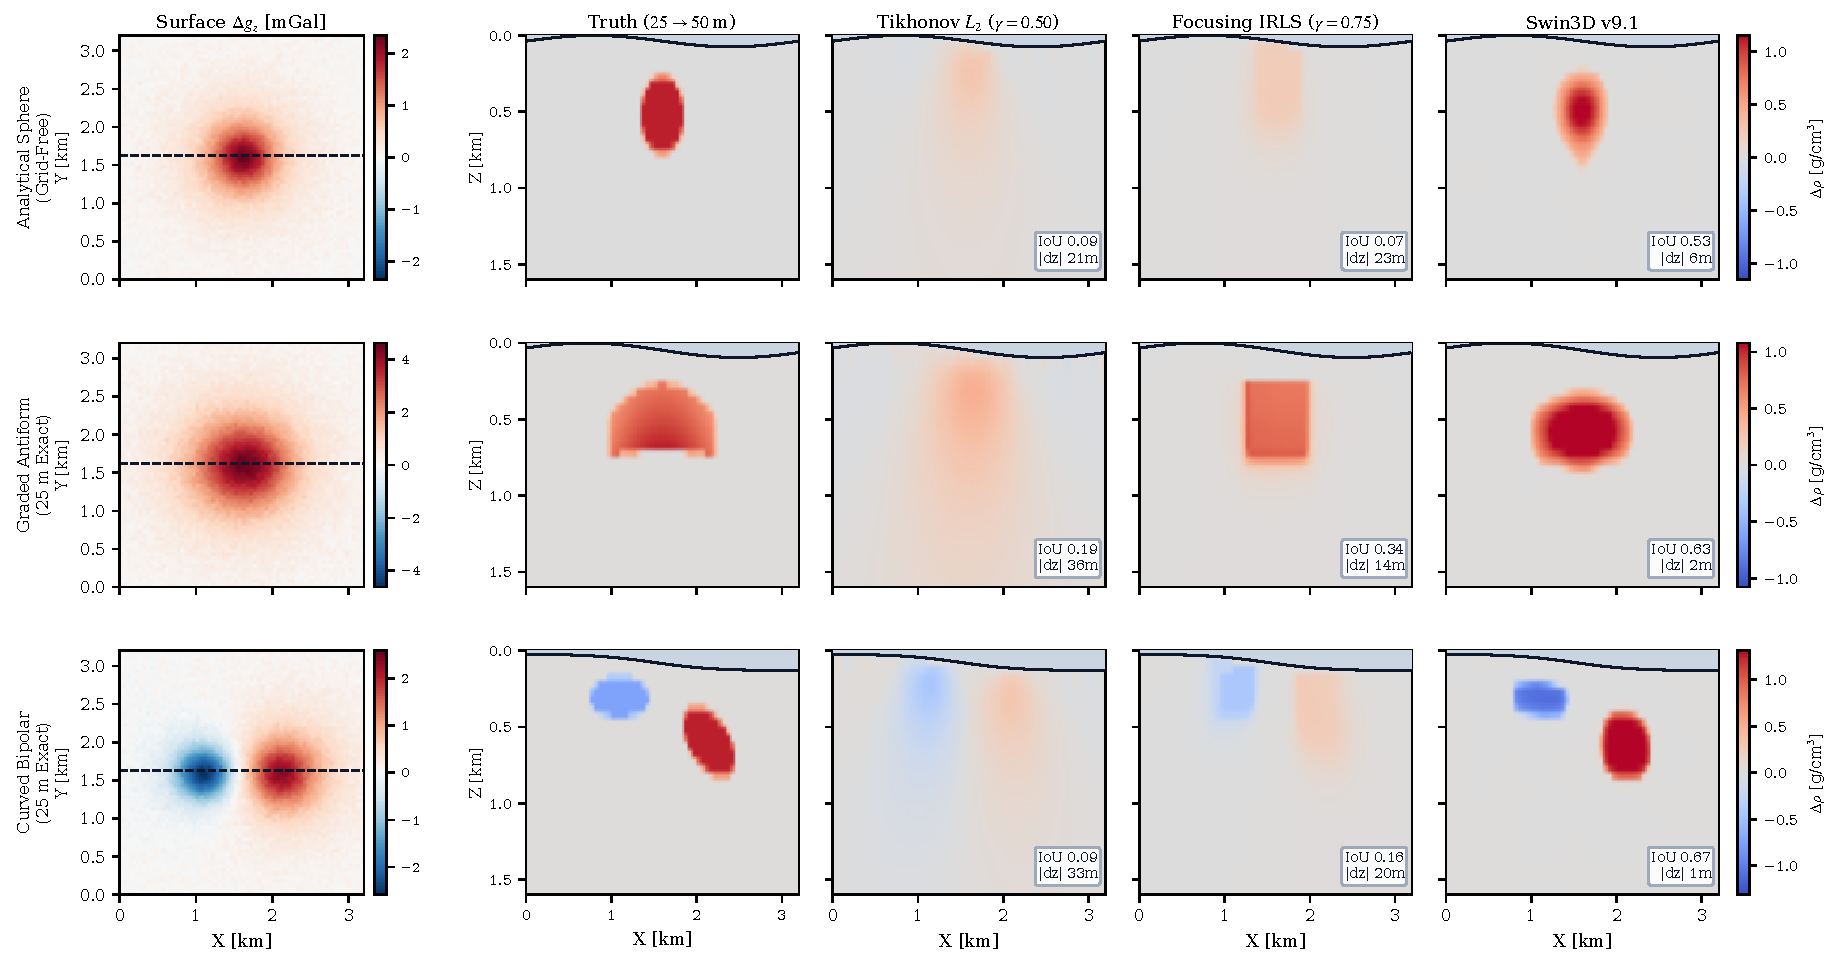
\includegraphics[width=\textwidth]{figures/fig4_ood_noninversecrime.pdf}
  \caption{Independent non-inverse-crime out-of-distribution (OOD) benchmark comparison (2\% white noise). Surface gravity fields are generated via the exact grid-free analytical sphere formula (Row~1) and direct exact Nagy prism summation on a $25$\,m fine mesh at exact station heights (Rows~2--3), bypassing the $50$\,m training FFT operator entirely. Column~2 shows volume-averaged $25\to 50$\,m ground truth.}
  \label{fig:ood}
\end{figure*}

\begin{table}[t]
\centering
\caption{Independent non-inverse-crime out-of-distribution (OOD) benchmark comparison (2\% white Gaussian noise). Forward anomalies are synthesized without the $50$\,m training operator: an exact closed-form analytical sphere and two continuous curved/depth-graded structures integrated via direct exact Nagy prism summation on a $2\times$ finer $25$\,m mesh ($128\times 128\times 64$) at exact station elevations. Bold marks best per benchmark.}
\label{tab:ood}
\small
\setlength{\tabcolsep}{4pt}
\resizebox{\textwidth}{!}{%
\begin{tabular}{llcccccccc}
\toprule
Benchmark & Method & IoU $\uparrow$ & RMSE $\downarrow$ & $\text{SSIM}_{d_3}$ $\uparrow$ & $|\Delta z|$ [m] $\downarrow$ & Amp. $\to 1$ & Misfit [\%] $\downarrow$ & $\chi^2_{\mathrm{red}}$ $\to 1$ & Time [s] $\downarrow$ \\
\midrule
\multirow{3}{*}{Analytical Sphere (Grid-Free)} & Tikhonov $L_2$ ($\gamma=0.50$) & 0.094 & 0.065 & 0.111 & 21.4 & 0.177 & 3.33 & 0.72 & 2.18 \\
 & Focusing IRLS ($\gamma=0.75$) & 0.068 & 0.062 & 0.183 & 22.8 & 0.190 & 6.04 & 1.26 & 7.03 \\
 & \texttt{Swin3D v9.1} & \textbf{0.532} & \textbf{0.030} & \textbf{0.728} & \textbf{5.9} & \textbf{0.779} & \textbf{1.65} & \textbf{0.98} & \textbf{0.19} \\
\midrule
\multirow{3}{*}{Graded Antiform (25 m Exact)} & Tikhonov $L_2$ ($\gamma=0.50$) & 0.186 & 0.089 & 0.181 & 35.6 & 0.336 & 2.52 & 0.72 & 2.90 \\
 & Focusing IRLS ($\gamma=0.75$) & 0.344 & 0.072 & 0.375 & 14.3 & 0.648 & 4.24 & 1.32 & 9.19 \\
 & \texttt{Swin3D v9.1} & \textbf{0.625} & \textbf{0.057} & \textbf{0.664} & \textbf{1.5} & \textbf{0.937} & \textbf{1.34} & \textbf{1.05} & \textbf{0.24} \\
\midrule
\multirow{3}{*}{Curved Bipolar (25 m Exact)} & Tikhonov $L_2$ ($\gamma=0.50$) & 0.095 & 0.083 & 0.245 & 32.8 & 0.254 & \textbf{3.11} & 0.72 & 4.53 \\
 & Focusing IRLS ($\gamma=0.75$) & 0.162 & 0.079 & 0.354 & 20.2 & 0.277 & 5.53 & 1.35 & 10.49 \\
 & \texttt{Swin3D v9.1} & \textbf{0.670} & \textbf{0.047} & \textbf{0.795} & \textbf{1.4} & \textbf{0.976} & 4.22 & \textbf{1.23} & \textbf{0.20} \\
\midrule
\multirow{3}{*}{\textbf{Mean (3 Benchmarks)}} & Tikhonov $L_2$ ($\gamma=0.50$) & 0.125 & 0.079 & 0.179 & 29.9 & 0.255 & 2.99 & 0.72 & 3.20 \\
 & Focusing IRLS ($\gamma=0.75$) & 0.192 & 0.071 & 0.304 & 19.1 & 0.372 & 5.27 & 1.31 & 8.90 \\
 & \texttt{Swin3D v9.1} & \textbf{0.609} & \textbf{0.045} & \textbf{0.729} & \textbf{2.9} & \textbf{0.897} & \textbf{2.40} & \textbf{1.09} & \textbf{0.21} \\
\bottomrule
\end{tabular}%
}
\end{table}


Across all three non-inverse-crime tests, \texttt{Swin3D v9.1} generalizes cleanly without fine-tuning: it achieves IoU \valOodSwinSphIoU{} ($|\Delta z|=\valOodSwinSphDz{}$\,m) vs.\ Focusing IRLS \valOodFocSphIoU{} on the grid-free sphere; IoU \valOodSwinDomeIoU{} ($|\Delta z|=\valOodSwinDomeDz{}$\,m) vs.\ \valOodFocDomeIoU{} on the continuously depth-graded antiform; and IoU \valOodSwinBipIoU{} ($|\Delta z|=\valOodSwinBipDz{}$\,m) vs.\ \valOodFocBipIoU{} on the curved tilted bipolar pair. Across the OOD suite, \texttt{Swin3D v9.1} raises mean IoU from \valOodMeanTikIoU{} (Tikhonov) and \valOodMeanFocIoU{} (Focusing IRLS) to \valOodMeanSwinIoU{} while cutting mean $|\Delta z|$ from \valOodMeanTikDz{}\,m and \valOodMeanFocDz{}\,m down to \valOodMeanSwinDz{}\,m. On the smoothly graded antiform (Row~2), note that the lithology prototype prior mildly homogenizes the interior gradient toward a uniform dense core---an instructive inductive bias to refine in future continuous-density work.

\begin{figure*}[t]
  \centering
  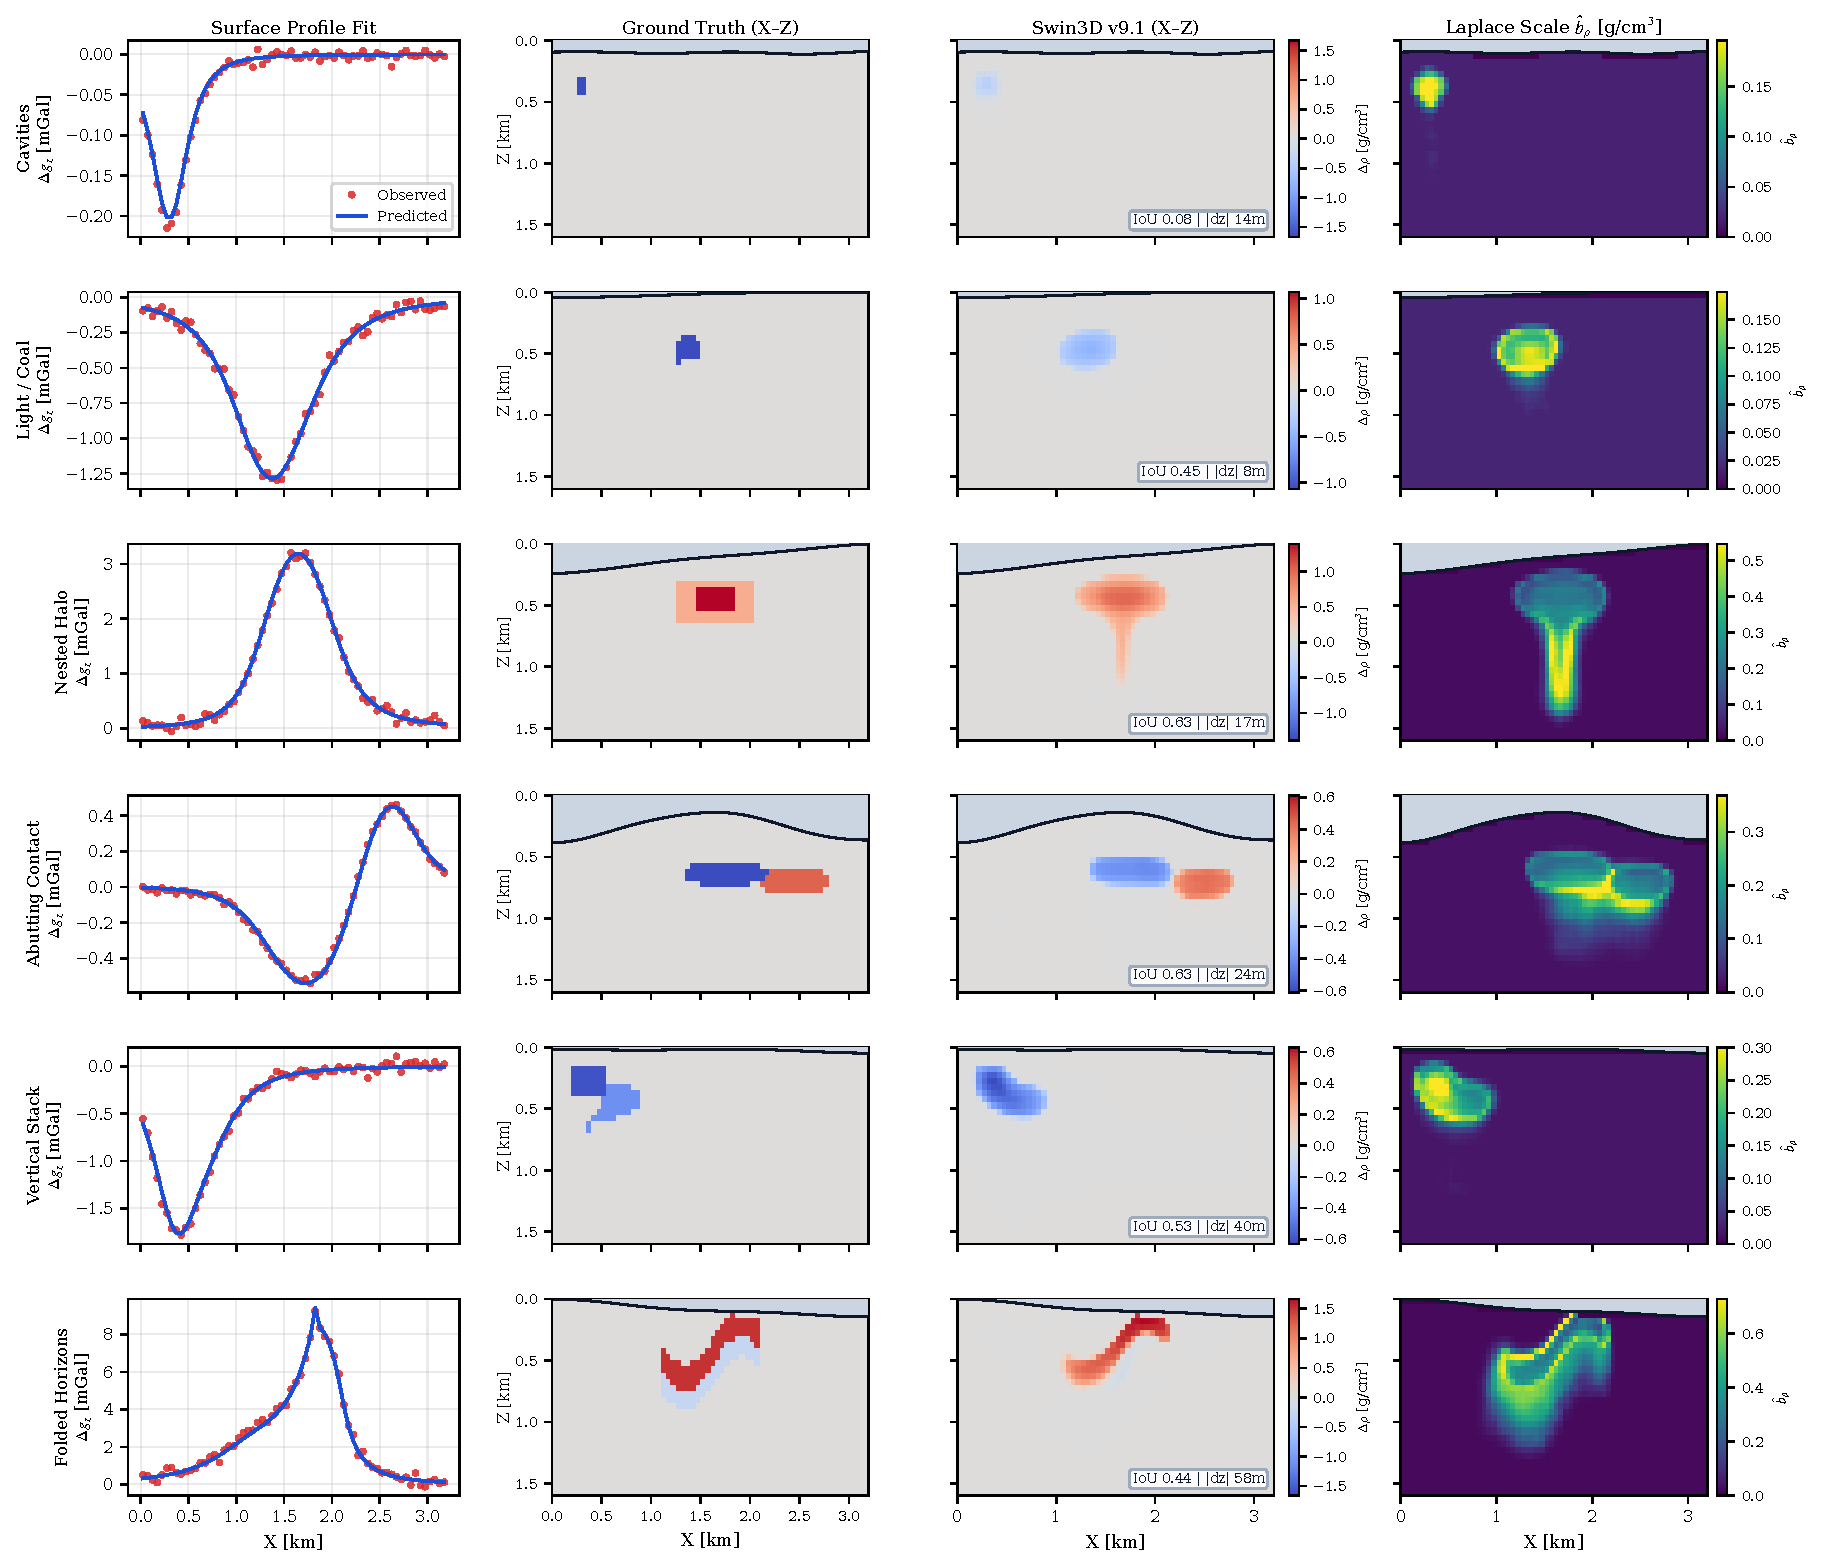
\includegraphics[width=\textwidth]{figures/fig5_showcase_composite.pdf}
  \caption{Six held-out multi-lithology archetypes (disjoint seed~40260, fixed 2\% white Gaussian noise, raw un-detrended mode): Surface gravity profile fit (Col.~1), Ground Truth $X$--$Z$ (Col.~2), Predicted $\Delta\hat{\rho}$ (Col.~3), and air-masked Laplace scale $\hat{b}_\rho$ (Col.~4).}
  \label{fig:showcase}
\end{figure*}

Figure~\ref{fig:showcase} complements the canonical and OOD comparisons across six held-out procedural phenotypes at fixed 2\% white noise (raw un-detrended mode, interior cross-sections): a tiny edge-adjacent cavity ($\text{IoU }\valShowZeroIoU{}, |\Delta z|=\valShowZeroDz{}\,$m), light coal seam ($\text{IoU }\valShowOneIoU{}, |\Delta z|=\valShowOneDz{}\,$m), nested core--halo ($\text{IoU }\valShowTwoIoU{}, |\Delta z|=\valShowTwoDz{}\,$m), abutting positive/negative contacts ($\text{IoU }\valShowThreeIoU{}, |\Delta z|=\valShowThreeDz{}\,$m), vertical stack ($\text{IoU }\valShowFourIoU{}, |\Delta z|=\valShowFourDz{}\,$m), and folded strata ($\text{IoU }\valShowFiveIoU{}, |\Delta z|=\valShowFiveDz{}\,$m). Two diagnostic insights stand out: (i) predicted Laplace scale $\hat{b}_\rho$ (Col.~4, masked to active subsurface voxels) accurately traces contact shells, abutting interfaces, and poorly constrained deep undersides; and (ii) in Row~1 (\emph{Cavities}), an uncurated tiny 2-cell void located near the left domain boundary ($X \approx 0.3$\,km, peak anomaly $-0.20$\,mGal) loses amplitude recovery (IoU \valShowZeroIoU{}) even though depth is localized within \valShowZeroDz{}\,m and $\hat{b}_\rho$ sharply flags elevated uncertainty right over the void.

\subsection{Noise Sensitivity, Depth Resolution, Clearance, and Laplace Calibration}

\begin{figure*}[t]
  \centering
  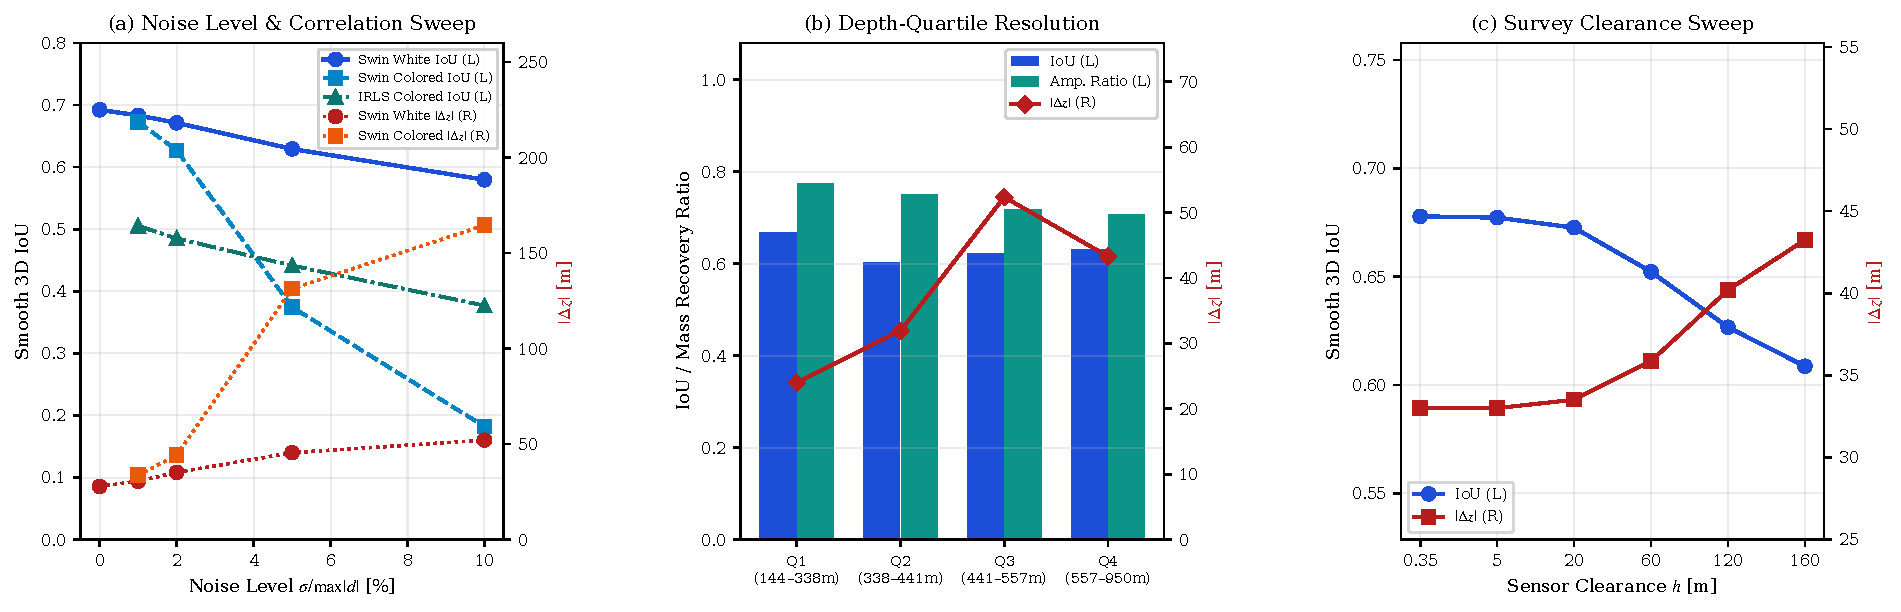
\includegraphics[width=\textwidth]{figures/fig6_sensitivity_depth.pdf}
  \caption{Robustness and physical resolution limits. (a) Sensitivity to white Gaussian noise vs.\ spatially correlated noise ($\sigma_c = 1.5\,\Delta x = 75$\,m) on $N=\valNNoise{}$ ground scenes for \texttt{Swin3D v9.1} alongside paired classical Focusing IRLS ($N=\valNIrlsNoise{}$) on correlated noise, revealing a crossover above 3--4\% colored noise. (b) Depth-quartile performance on the $N=\valNBucketTotal{}$ held-out test suite. (c) Paired sensor-clearance sweep ($h=0.35\text{--}160$\,m at 1.5\% white noise) on the exact same $N=\valNNoise{}$ ground scenes.}
  \label{fig:sens_depth}
\end{figure*}

\begin{table}[t]
\centering
\caption{Sensitivity to surface measurement noise level and spatial correlation on unified ground-survey scenes ($N=\valNNoise{}$ for \texttt{Swin3D v9.1}, and a paired $N=\valNIrlsNoise{}$ subset for classical Focusing IRLS). White Gaussian noise is compared against spatially smoothed colored noise ($\sigma_c = 1.5\,\Delta x = 75$\,m).}
\label{tab:noise}
\small
\setlength{\tabcolsep}{4.5pt}
\resizebox{\textwidth}{!}{%
\begin{tabular}{llcccccccc}
\toprule
Method & Noise Type & $\sigma / \max|d|$ & IoU (mean\,$\pm$\,std) $\uparrow$ & RMSE $\downarrow$ & $\text{SSIM}_{d_3}$ $\uparrow$ & $|\Delta z|$ [m] $\downarrow$ & Amp. $\to 1$ & Misfit [\%] $\downarrow$ & $\chi^2_{\mathrm{red}}$ \\
\midrule
\multirow{5}{*}{\texttt{Swin3D v9.1}} & \multirow{5}{*}{White Gaussian} & 0\% & 0.692\,$\pm$\,0.153 & 0.067 & 0.651 & 27.8 & 0.804 & 4.08 & --- \\
 &  & 1\% & 0.683\,$\pm$\,0.160 & 0.068 & 0.642 & 30.6 & 0.800 & 3.61 & 2.74 \\
 &  & 2\% & 0.671\,$\pm$\,0.153 & 0.072 & 0.621 & 35.2 & 0.792 & 3.56 & 1.43 \\
 &  & 5\% & 0.629\,$\pm$\,0.151 & 0.082 & 0.564 & 45.5 & 0.765 & 4.25 & 1.07 \\
 &  & 10\% & 0.580\,$\pm$\,0.176 & 0.089 & 0.500 & 52.1 & 0.709 & 6.97 & 1.04 \\
\midrule
\multirow{4}{*}{\texttt{Swin3D v9.1}} & \multirow{4}{*}{Correlated ($\sigma_c=1.5\Delta x$)} & 1\% & 0.673\,$\pm$\,0.160 & 0.070 & 0.622 & 33.7 & 0.796 & 4.34 & 2.69 \\
 &  & 2\% & 0.627\,$\pm$\,0.178 & 0.077 & 0.565 & 44.2 & 0.775 & 5.87 & 1.47 \\
 &  & 5\% & 0.375\,$\pm$\,0.227 & 0.110 & 0.351 & 131.4 & 0.493 & 22.06 & 2.28 \\
 &  & 10\% & 0.182\,$\pm$\,0.142 & 0.152 & 0.189 & 164.6 & 0.310 & 52.73 & 2.92 \\
\midrule
\multirow{4}{*}{Focusing IRLS ($N=\valNIrlsNoise{}$)} & \multirow{4}{*}{Correlated ($\sigma_c=1.5\Delta x$)} & 1\% & 0.505\,$\pm$\,0.067 & 0.178 & 0.326 & 94.9 & 0.701 & 2.58 & 1.19 \\
 &  & 2\% & 0.485\,$\pm$\,0.080 & 0.190 & 0.306 & 110.5 & 0.698 & 4.46 & 1.07 \\
 &  & 5\% & 0.441\,$\pm$\,0.102 & 0.223 & 0.264 & 177.3 & 0.687 & 8.63 & 0.98 \\
 &  & 10\% & 0.377\,$\pm$\,0.123 & 0.264 & 0.203 & 294.4 & 0.629 & 15.47 & 1.27 \\
\bottomrule
\end{tabular}%
}
\end{table}

\begin{table}[t]
\centering
\caption{Depth-quartile resolution across the $N=\valNBucketTotal{}$ validation suite (Panel~A) and paired sensor-clearance sweep at fixed 1.5\% noise ($N=\valNNoise{}$, Panel~B).}
\label{tab:depth_clearance}
\small
\setlength{\tabcolsep}{5.5pt}
\resizebox{\textwidth}{!}{%
\begin{tabular}{lccccccc}
\toprule
Sub-group / Regime & $N$ & IoU $\uparrow$ & RMSE $\downarrow$ & $\text{SSIM}_{d_3}$ $\uparrow$ & $|\Delta z|$ [m] $\downarrow$ & Amp. $\to 1$ & Misfit [\%] $\downarrow$ \\
\midrule
\multicolumn{8}{l}{\textit{Panel A: Source Depth Quartiles (mass-weighted depth below terrain)}} \\
Q1 (183--340\,m) & 32 & 0.678 & 0.063 & 0.615 & 22.2 & 0.810 & 5.81 \\
Q2 (340--459\,m) & 32 & 0.638 & 0.082 & 0.551 & 43.0 & 0.757 & 5.46 \\
Q3 (459--537\,m) & 32 & 0.573 & 0.066 & 0.551 & 45.2 & 0.686 & 6.28 \\
Q4 (537--984\,m) & 32 & 0.517 & 0.082 & 0.555 & 47.2 & 0.618 & 6.42 \\
\midrule
\multicolumn{8}{l}{\textit{Panel B: Paired Survey Clearance Height Above Terrain}} \\
Clearance $h = 0.35$\,m & 24 & 0.606 & 0.047 & 0.651 & 36.2 & 0.718 & 3.72 \\
Clearance $h = 5$\,m & 24 & 0.606 & 0.047 & 0.650 & 35.9 & 0.718 & 3.66 \\
Clearance $h = 20$\,m & 24 & 0.605 & 0.047 & 0.649 & 35.6 & 0.716 & 3.59 \\
Clearance $h = 60$\,m & 24 & 0.598 & 0.048 & 0.643 & 37.6 & 0.710 & 3.51 \\
Clearance $h = 120$\,m & 24 & 0.583 & 0.049 & 0.625 & 39.6 & 0.695 & 3.68 \\
Clearance $h = 160$\,m & 24 & 0.570 & 0.050 & 0.609 & 40.9 & 0.683 & 4.66 \\
\bottomrule
\end{tabular}%
}
\end{table}


\paragraph{White vs.\ Spatially Correlated Noise (and Classical Crossover).}
Table~\ref{tab:noise} and Figure~\ref{fig:sens_depth}(a) evaluate $N=\valNNoise{}$ ground scenes perturbed by zero-mean white Gaussian noise versus spatially smoothed colored noise ($\sigma_c = 1.5\,\Delta x = 75$\,m Gaussian blur normalized to equal variance), together with paired classical Focusing IRLS runs ($N=\valNIrlsNoise{}$ subset). Under white noise from $0\%$ to $10\%$ of peak signal, \texttt{Swin3D v9.1} degrades smoothly and monotonically: IoU moves from \valNoiseZeroIoU{} ($0\%$) to \valNoiseFiveWhiteIoU{} ($5\%$) and \valNoiseTenWhiteIoU{} ($10\%$), while $|\Delta z|$ remains bounded within \valNoiseTenWhiteDz{}\,m ($\approx 1$ voxel). Under \textbf{spatially correlated noise}, however, a stark regime crossover emerges: at $1\text{--}2\%$ colored noise, \texttt{Swin3D v9.1} clearly leads Focusing IRLS (IoU \valNoiseOneColoredIoU{}--\valNoiseTwoColoredIoU{}, $|\Delta z|=\valNoiseOneColoredDz{}$--\valNoiseTwoColoredDz{}\,m), whereas at $5\%$ and $10\%$ colored noise \texttt{Swin3D v9.1} drops sharply to \valNoiseFiveColoredIoU{} and \valNoiseTenColoredIoU{} IoU ($|\Delta z|=\valNoiseFiveColoredDz{}$--\valNoiseTenColoredDz{}\,m) and is \textbf{overtaken by classical Focusing IRLS} (\valIrlsTenColoredIoU{} IoU at $10\%$ colored noise, though IRLS incurs $|\Delta z|=\valIrlsTenColoredDz{}$\,m). Physically, smooth $75$\,m lateral perturbations mimic real intermediate-wavelength gravitational anomalies from deep bodies along the $1/r^2$ manifold, confirming that variogram-aware pre-whitening or high-pass filtering is mandatory whenever coherent drift exceeds $2\%$ of peak anomaly amplitude.

\paragraph{Depth-Quartile Resolution and Reconciled Sensor Clearance.}
Table~\ref{tab:depth_clearance} and Figure~\ref{fig:sens_depth}(b)--(c) isolate geometric attenuation. Across depth quartiles of the $N=\valNBucketTotal{}$ held-out suite (Panel~A), shallow quartile Q1 (\valQOneRange{}\,m) reaches IoU \valQOneIoU{}, $|\Delta z| = \valQOneDz{}$\,m, and mass recovery \valQOneAmp{}, transitioning gradually to deep quartile Q4 (\valQFourRange{}\,m) at IoU \valQFourIoU{}, $|\Delta z| = \valQFourDz{}$\,m, and mass recovery \valQFourAmp{}, while $\text{SSIM}_{d_3}$ holds tightly within \valQMinSSIMd{}--\valQMaxSSIMd{}. On the exact same $N=\valNNoise{}$ ground scenes as Table~\ref{tab:noise} at fixed $1.5\%$ white noise (Panel~B), ground clearance $h=0.35$\,m attains IoU \valClrGroundIoU{} (matching the $1\%\text{--}2\%$ white-noise bracket seamlessly), stays virtually flat through $20$\,m (\valClrTwentyIoU{}), and degrades mildly to \valClrHighIoU{} IoU and \valClrHighDz{}\,m depth error at $160$\,m airborne altitude.

\begin{figure*}[t]
  \centering
  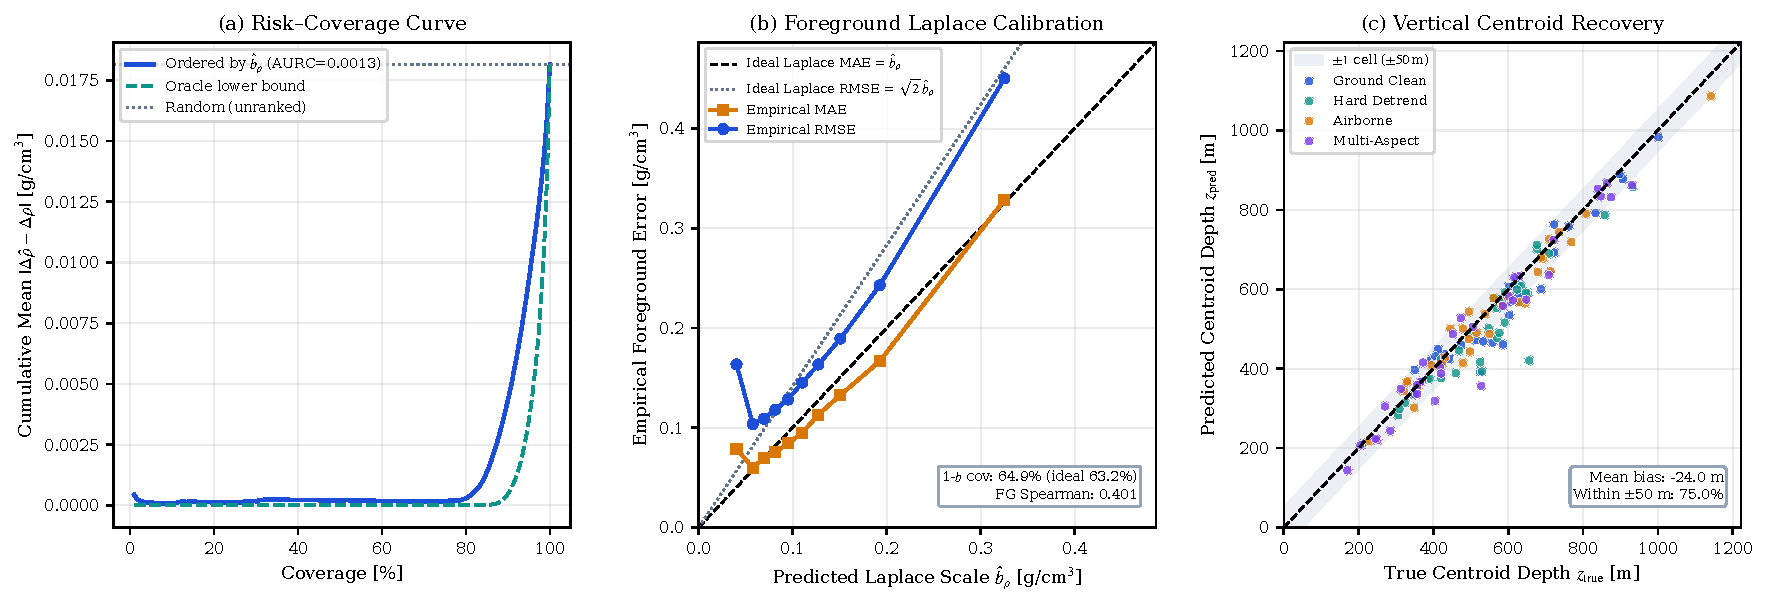
\includegraphics[width=\textwidth]{figures/fig7_uncertainty_calib.pdf}
  \caption{Laplace uncertainty calibration and centroid recovery across $N=\valNBucketTotal{}$ held-out volumes (seed~\valTestSeed{}). (a) Selective-prediction Risk--Coverage curve sorted by predicted Laplace scale $\hat{b}_\rho$ (exact pooled $\mathrm{AURC} = \valCompAURCPooled{}$). (b) Binned foreground empirical MAE and RMSE versus predicted $\hat{b}_\rho$ compared against theoretical Laplace expectations ($\text{MAE}=\hat{b}_\rho$, $\text{RMSE}=\sqrt{2}\,\hat{b}_\rho$; $1$-$b$ coverage \valCompFgCov{}\% vs.\ ideal $63.2\%$, foreground Spearman $\rho_{\mathrm{fg}}=\valCompFgUncSp{}$). (c) Global predicted vs.\ true centroid depth across all four regimes ($\pm 50$\,m corridor shaded; mean signed bias $\valCompCentroidBias{}$\,m, \valCompCentroidWithinFifty{}\% within $\pm 50$\,m).}
  \label{fig:calib}
\end{figure*}

\paragraph{Laplace Uncertainty Calibration and Failure Modes.}
Figure~\ref{fig:calib} evaluates the heteroscedastic Laplace $\beta$-NLL head across all $N=\valNBucketTotal{}$ held-out volumes. Ordering subsurface voxels by $\hat{b}_\rho$ (Figure~\ref{fig:calib}(a)) tracks the post-hoc error oracle closely, attaining exact pooled $\mathrm{AURC} = \valCompAURCPooled{}\;\text{g/cm}^3$ (all-subsurface Spearman $\rho_{\mathrm{all}} = \valCompUncSp{}$). Within ground-truth foreground bodies (Figure~\ref{fig:calib}(b), foreground Spearman $\rho_{\mathrm{fg}} = \valCompFgUncSp{}$), empirical MAE aligns closely with the theoretical Laplace diagonal $\text{MAE} = \hat{b}_\rho$ across deciles 2--10 while empirical RMSE tracks $\sqrt{2}\,\hat{b}_\rho$, achieving $1$-$b$ coverage of \valCompFgCov{}\% (close to the theoretical Laplace $63.2\%$) and a 1-cell boundary calibration ratio $\overline{\hat{b}_\rho}_{\partial\mathcal{B}} / \overline{|\Delta\hat{\rho}-\Delta\rho|}_{\partial\mathcal{B}} = \valCompBdRatio{}$ (ideal $1.00$). Two caveats must be stated candidly: (i) in the lowest-scale foreground decile ($\hat{b}_\rho \approx 0.04$), empirical error exhibits mild non-monotonic under-dispersion from missed faint margins, and on isolated sharp canonical targets (e.g., Compact Ore Block and Dipping Dyke) foreground $1$-$b$ coverage drops sharply (\valCanonSwinOreCov{}\% and \valCanonSwinDykeCov{}\%, and \valCleanHardXferCov{}\% under zero-shot clean transfer) because amplitude underestimation shifts entire body interiors uniformly beyond $\hat{b}_\rho$; and (ii) Figure~\ref{fig:calib}(c) reveals a modest systematic shallow bias of $\valCompCentroidBias{}$\,m across the \valNBucketTotal{} held-out scenes, with \valCompCentroidWithinFifty{}\% falling within the $\pm 1$-voxel ($\pm 50$\,m) corridor.

%======================================================================
\section{Deployment Efficiency and Discussion}
\label{sec:deploy_discuss}
%======================================================================

\subsection{Matched-Thread ONNX and CoreML Production Performance}

\begin{table}[t]
\centering
\caption{Single-volume ($64\times 64\times 32$) median wall-clock runtime and ONNX numerical parity on a MacBook Air (Apple~M4, 32\,GB unified memory). Neural timings report the median of 10 runs; classical timings report the median across the 4 canonical benchmarks in Table~\ref{tab:canonical}, all constrained to \valCpuThreads{} CPU threads for matched comparison.}
\label{tab:timing}
\small
\setlength{\tabcolsep}{6pt}
\resizebox{\textwidth}{!}{%
\begin{tabular}{@{}lccc@{}}
\toprule
Solver / Execution Backend & Median Runtime & Speedup vs.\ IRLS & Max Rel.\ Parity Diff \\
\midrule
\texttt{Swin3D v9.1} (ONNX CoreML ANE/CPU) & 103.1\,ms & 99$\times$ & 1.02e-02 \\
\texttt{Swin3D v9.1} (ONNX Runtime CPU, 4 threads) & 172.1\,ms & 59$\times$ & 6.34e-06 \\
\texttt{Swin3D v9.1} (PyTorch CPU, 4 threads) & 185.7\,ms & 55$\times$ & Reference \\
Tikhonov $L_2$ (Python/PyTorch FFT, 10 iters, 4 threads) & 3.64\,s & 2.8$\times$ & --- \\
Focusing IRLS (Python/PyTorch FFT, 12 iters, 4 threads) & 10.17\,s & 1.0$\times$ & --- \\
\bottomrule
\end{tabular}%
}
\end{table}


Table~\ref{tab:timing} benchmarks single-volume ($64\times 64\times 32$) median wall-clock latency and numerical parity on the MacBook Air (Apple~M4, 32\,GB unified memory), constraining PyTorch CPU, ONNX Runtime CPU, and the Python/PyTorch FFT classical solvers uniformly to \valCpuThreads{} CPU threads for a fair comparison. Exporting \texttt{PotentialFieldTransformer3DV9} (opset-17, \valOnnxNodes{} raw ONNX ops before runtime graph optimization, outputting dual $(\Delta\hat{\rho}, \hat{s})$ tensors) to ONNX Runtime CPU achieves \valTimeOnnxCpuMs{}\,ms median latency (\valTimePtMs{}\,ms in PyTorch CPU)---\valSpeedupOnnxVsFoc{} faster than 12-iteration Python/PyTorch FFT Focusing IRLS (\valTimeFocS{}\,s)---at \valTimeOnnxCpuDiff{} maximum relative parity difference. Enabling Apple's \texttt{CoreMLExecutionProvider} (\texttt{CPUAndNeuralEngine}) offloads 1,449 of 1,508 optimized runtime graph nodes across 17 Neural Engine/CPU partitions (directly enabled by the FFT-free \texttt{OddPyramidGravity} design), accelerating inference to \valTimeCoremlMs{}\,ms (\valSpeedupCoremlVsFoc{} speedup) with \valTimeCoremlDiff{} maximum relative difference under FP16 accelerator arithmetic. We note explicitly that classical timings reflect our Python/PyTorch FFT implementation rather than an optimized native C++ binary, so speedups relative to multi-threaded C++ solvers would be narrower while still leaving neural inference firmly in the $\sim 100\text{--}200$\,ms interactive regime inside \texttt{Mod3D} \citep{cerovsky_mod3d}.

\subsection{Physical Mechanisms, Key Limitations, and Future Work}

\paragraph{Physics-in-the-Loop Attention vs.\ Classical Focusing.}
Classical depth-weighted Tikhonov $L_2$ and focusing IRLS solvers enforce only generic smoothness or compactness priors; consequently, they struggle when dipping sheets or opposing polarities produce interfering gravity signatures, yet focusing IRLS retains a clear advantage on near-surface outcropping basins (Table~\ref{tab:canonical}, Row~4) and high-amplitude spatially correlated noise (Table~\ref{tab:noise}). Embedding two frozen spatial-pyramid forward/adjoint residual stages directly inside a 3D Swin+axial backbone lets \texttt{Swin3D v9.1} reconcile global lateral gravity tails with local 3D lithology contacts while transferring cleanly to grid-free analytical and $25$\,m fine-mesh OOD targets (Table~\ref{tab:ood}). Equally important, our chronological progression analysis (Table~\ref{tab:ablation}) clarifies that long multi-regime training (\valVNineOneEp{} epochs) and unified Stage-2 decoding work synergistically; attributing the full Panel~A gain solely to decoder architecture without epoch matching would overstate the architectural delta.

\paragraph{Limitations and Roadmap Toward Field Surveys.}
Four key limitations bound the present work and define concrete directions for future research:
\begin{enumerate}[leftmargin=1.4em,itemsep=0.25em]
  \item \emph{Absence of Field Validation \& Conditioning Prerequisites:} Because calibrated field gravity datasets were inaccessible here, complex real-world effects---strong lateral petrophysical heterogeneity outside our 7 lithology classes, irregular station gridding, and non-linear regional gravity interference beyond border planes---remain empirically untested. Preparing field surveys for standalone inference will require standard complete Bouguer terrain reduction, consistent regional trend removal, variogram-based pre-whitening whenever spatially coherent drift exceeds $2\%$ of peak anomaly amplitude (Section~\ref{sec:experiments}), and accurate survey clearance/aspect metadata keeping relief $\le 25\%$ of grid depth.
  \item \emph{Direct Deep-Learning Baselines:} While we benchmark thoroughly against classical $L_2$ and Focusing IRLS solvers across both in-distribution and non-inverse-crime OOD targets plus our own \texttt{v3}--\texttt{v9.1} progression, we did not re-train a matched-budget 3D U-Net/CNN or re-implement \citet{yu2025swin} (whose code is unavailable) on our topographic ground-to-airborne multi-regime curriculum. Establishing a controlled matched-epoch 3D CNN vs.\ Swin benchmark remains a high-priority follow-up.
  \item \emph{Planar-Earth Approximation, Edge Truncation, and Lithology Bounds:} Both the training FFT operator and \texttt{OddPyramidGravity} assume flat Cartesian layers over local/regional apertures ($3.2\text{--}10$\,km); anomalies intersecting the outer perimeter experience boundary truncation (as seen on the edge-adjacent cavity in Figure~\ref{fig:showcase}), and continental extents require spherical tesseroid operators \citep{uieda2016}. In addition, the 7-class lithology mixture gently biases interiors toward piecewise-constant bands inside $[-2.67, +1.95]\;\text{g/cm}^3$ (visible on the graded antiform in Figure~\ref{fig:ood}) and exhibits under-dispersed uncertainty on isolated sharp blocks where uniform amplitude attenuation dominates, pointing toward conformal calibration or deep ensembles for quantitative risk budgeting.
  \item \emph{Magnetic and Gradiometry Extensions:} Replacing the scalar vertical Nagy kernel in~\eqref{eq:forward_nagy} with vector magnetic dipole kernels (passing inclination/declination into \texttt{scale\_mlp}) or gravity gradient tensor kernels extends the same physics-coupled Swin framework directly to 3D magnetic susceptibility and joint multi-physics inversion.
\end{enumerate}

%======================================================================
\section{Conclusion and Reproducibility}
\label{sec:conclusion}
%======================================================================

We presented \texttt{Swin3D v9.1}, a physics-coupled hierarchical 3D Shifted-Window and axial Transformer for ground and airborne vertical gravity inversion over undulating topography integrating a fixed 19-channel derivative stem, additive 9-D survey conditioning, vertical Green's attention biases, 7-class lithology prototype cross-attention, two frozen spatial-pyramid forward/adjoint residual stages, and a zone-stratified Laplace $\beta$-NLL uncertainty head. Evaluated on strictly disjoint held-out multi-regime test benchmarks ($N=\valNBucketTotal{}$, seed~\valTestSeed{}), four canonical targets, and three independent non-inverse-crime analytical and $25$\,m fine-mesh OOD benchmarks, \texttt{Swin3D v9.1} achieves strong volumetric accuracy (\valCompIoU{} held-out composite IoU; \valOodMeanSwinIoU{} OOD IoU with \valOodMeanSwinDz{}\,m mean centroid error) and calibrated foreground Laplace MAE tracking while executing in \valTimeOnnxCpuMs{}\,ms on CPU (\valSpeedupOnnxVsFoc{} speedup vs.\ Python/PyTorch FFT Focusing IRLS) and \valTimeCoremlMs{}\,ms on Apple CoreML Neural Engine (\valSpeedupCoremlVsFoc{} speedup). At the same time, our controlled stress tests clearly delineate practical boundaries---most notably vulnerability to spatially correlated noise above $2\%$, mild $\valCompCentroidBias{}$\,m shallow centroid bias, and reduced $1$-$b$ coverage on isolated sharp blocks---providing a transparent foundation for future field validation and controlled CNN/Transformer benchmarking.

\paragraph{Code, Frozen Checkpoints, and One-Command Reproducibility.}
All neural architectures, forward physics simulators, classical solvers, and ONNX export wrappers are released openly inside \texttt{Mod3D} at \url{https://github.com/igorcerovsky/Mod3D/tree/main/.inv}, alongside an interactive WebGL2 modeling demo at \url{https://igorcerovsky.github.io/Mod3D/}. Every checkpoint evaluated in this manuscript (including flagship \texttt{v9.1\_hard\_best.pt} at epoch~\valVNineOneEp{} and all \texttt{v3}--\texttt{v9.1} progression models) is archived in \texttt{.inv/paper/models/} with SHA-256 checksums and full configuration metadata in \texttt{MODEL\_METADATA.json}. Every metric, macro, table, and vector figure in this manuscript is regenerated deterministically via \texttt{.inv/paper/scripts/update\_paper.sh}.

\section*{Acknowledgments}
The author thanks colleagues in potential-field geophysics and computer vision whose foundational work inspired this synthesis of potential-field physics with hierarchical 3D Transformers inside \texttt{Mod3D}. No external funding was received for this independent study.

\bibliographystyle{plainnat}
\bibliography{references}

\clearpage
%======================================================================
\appendix
\section{Architecture, Stem Features, and Compound Loss Specification}
\label{app:specs}
%======================================================================

To ensure full methodological reproducibility independent of reading source code, Tables~\ref{tab:app_arch}--\ref{tab:app_loss} summarize the exact architectural hyperparameters, fixed 19-channel stem features, 7 lithology density ranges, and compound loss components of \texttt{Swin3D v9.1} Base.

\begin{table}[ht]
\centering
\caption{Exact architectural dimensions and training hyperparameters of \texttt{Swin3D v9.1} Base (\valVNineOneParamsExact{} parameters).}
\label{tab:app_arch}
\small
\resizebox{\textwidth}{!}{%
\begin{tabular}{ll|ll}
\toprule
Architecture Parameter & Value & Training Hyperparameter & Value \\
\midrule
Canonical 3D grid $(N_z, N_x, N_y)$ & $(32, 64, 64)$ @ $50$\,m & Optimizer & AdamW ($\text{lr}=5\times 10^{-4}$) \\
2D encoder channels $(c_0, c_1, c)$ & $(32, 64, 128)$ & Schedule & Cosine + 10-ep warmup \\
3D token grid $(D_p, H_p, W_p)$ & $(8, 16, 16)$, patch $4$ & Batch size / steps per epoch & $8$ / $200$ ($1{,}600$ scenes/ep) \\
Transformer depth / heads & $6$ blocks / $4$ heads & Curriculum / dropout & $25$ epochs / $0.05$ \\
3D Swin window $(w_d, w_h, w_w)$ & $(8, 4, 4)$, shift $2$ & Precision / weight shadow & FP32 (MPS) / EMA \\
Lithology prototypes & $7\text{ classes} \times 3 = 21$ & Best checkpoint epoch & \valVNineOneEp{} (hard), \valVNineOneCleanEp{} (clean) \\
Decoder channels $(c_{\mathrm{mid}}, c_{\mathrm{vox}})$ & $(40, 24)$, depth $2$ & Train val / held-out test seed & \valTrainValSeed{} / \valTestSeed{} \\
\bottomrule
\end{tabular}%
}
\end{table}

\begin{table}[ht]
\centering
\caption{Fixed 19-channel geophysical stem features (zero learnable parameters) and 7-class lithology mixture bounds ($\text{g/cm}^3$ contrast relative to $2.67\;\text{g/cm}^3$ host rock).}
\label{tab:app_stem}
\small
\resizebox{\textwidth}{!}{%
\begin{tabular}{cl|cl}
\toprule
Ch.\ & Fixed Analytical Stem Feature & Class & Lithology Band ($\Delta\rho\;[\text{g/cm}^3]$) \\
\midrule
1--2 & Peak-normalized $g_n = \Delta g_z / s$; $\operatorname{asinh}(8 g_n)/\operatorname{asinh}(8)$ & 0 & Host background ($0.00$) \\
3--6 & Box-filter residuals $g_n - \operatorname{LP}_k(g_n)$, $k \in \{3, 9, 17, 25\}$ & 1 & Air cavity (fixed $-2.67$) \\
7--8 & $3\times 3$ FD Laplacian $g_{zz} = -(g_{xx}+g_{yy})$ (fine \& $\text{LP}_3$) & 2 & Water void (fixed $-1.67$) \\
9--11 & $|\nabla_h g_n|$; tilt-angle $\sin$; Euler depth proxy & 3 & Light / coal / evaporite ($[-1.60, -0.80]$) \\
12--14 & Structure-tensor coherence, $\cos 2\theta$, $\sin 2\theta$ & 4 & Sediments / waste ($[-0.85, -0.03]$) \\
15--18 & Valid mask ($2v-1$); terrain $4z_{\mathrm{terr}}$; terrain slope \& curv. & 5 & Mafic / intermediate ($[+0.03, +0.80]$) \\
19 & Detrending mode indicator ($2\,\text{dt} - 1$) & 6 & High-grade ore / ultramafic ($[+0.75, +1.95]$) \\
\bottomrule
\end{tabular}%
}
\end{table}

\begin{table}[ht]
\centering
\caption{Exact compound loss terms and scalar weights in~\eqref{eq:loss_total} for \texttt{Swin3D v9.1} (normalized contrast $p_n = \Delta\hat{\rho}/a$, $t_n = \Delta\rho/a$, $a=\max(0.05,\max|\Delta\rho|)$, depth ramp $w_z = 1 + 0.5\,z/Z_{\max}$).}
\label{tab:app_loss}
\small
\resizebox{\textwidth}{!}{%
\begin{tabular}{lll}
\toprule
Term & Weight & Exact Mathematical Formulation \\
\midrule
$\mathcal{L}_{\mathrm{struct}}$ & $1.00$ & $0.23(\mathcal{L}_{\mathrm{fg}} + \mathcal{L}_{\mathrm{rel}L_1} + \mathcal{L}_{\mathrm{IoU}} + \mathcal{L}_{\mathrm{grad}}) + 0.12\,\mathcal{L}_{\mathrm{band}} + \mathcal{L}_{\mathrm{halo}} + 0.05\,|S_{\mathrm{MGS}}(p_n)-S_{\mathrm{MGS}}(t_n)| + 0.08\,\mathcal{L}_{\mathrm{amp}}$ \\
$\mathcal{L}_{\mathrm{cls}}$ & $0.25$ & $0.50\,\text{CrossEntropy}(\hat{\mathbf{p}}_{\mathrm{cls}}, \mathbf{c}) + 0.50\,\text{Dice}(\hat{\mathbf{p}}_{\mathrm{cls}}, \mathbf{c}) + 0.25\,\text{AbsentClassLeak}$ \\
$\mathcal{L}_{\mathrm{coh}}$ & $0.12$ & $0.45\,\mathcal{L}_{\mathrm{incompat}} + 0.30\,\mathcal{L}_{\mathrm{cls\text{-}smooth}} + 0.25\,\mathcal{L}_{\mathrm{unit\text{-}purity}}$ (ties $\Delta\hat{\rho}$ to $\hat{\mathbf{p}}_{\mathrm{cls}}$) \\
$\mathcal{L}_{\mathrm{edt}}$ & $1.00$ & $0.25\,\text{SmoothL1}_{\beta=0.15}(\hat{\mathbf{e}}_{\mathrm{edt}}, \mathbf{e}_{\mathrm{edt}})$ on dilated foreground + contact mask \\
$\mathcal{L}_{\mathrm{coarse}}$ & $0.20$ & $0.50\,\text{SmoothL1}_{\beta=0.01} + 0.50\,\text{SoftIoU}$ on Stage-1 $(16\times 32\times 32)$ density $\Delta\hat{\rho}_1$ \\
$\mathcal{L}_{\mathrm{init}}$ & $0.10$ & $0.50\,\text{WeightedRel}L_1 + 0.50\,\text{Tversky}_{(0.35,0.65)}$ on Stage-2 pre-feedback $\Delta\rho_{\mathrm{init}}$ \\
$\mathcal{L}_{\mathrm{data}}$ & $0.50$ & $0.65\,\text{CharbRelRMSE}(\mathbf{G}\Delta\hat{\rho}-\mathbf{d}_{\mathrm{clean}}, \mathbf{d}_{\mathrm{clean}}) + 0.35\,\text{CharbRelGradRMSE}$ \\
$\mathcal{L}_{\beta\text{-NLL}}$ & $0.06$ & Zone-stratified Laplace $\beta$-NLL~\eqref{eq:betanll} ($\omega_{\mathrm{fg}}=0.50$, $\omega_{\mathrm{bd}}=0.35$, $\omega_{\mathrm{far}}=0.15$, $\beta_{\mathrm{NLL}}=0.5$) \\
\bottomrule
\end{tabular}%
}
\end{table}

\end{document}
